%这个是根据计算机学报官网下的LaTeX模板改的,主要修改内容:①把GBK编码改成了UTF-8编码。②引入zhwinfonts,用上传的字体文件实现了字体的使用。
%现存的问题:①中文无法使用加粗功能,但是英文可以。解决方式1:使用黑体来凑合代替。解决方式2:在PDF编辑器里面一个一个加粗。②无法实现模板中所要求的每页脚注从1开始的要求。
%如果您在使用该模板的过程中遇到问题,或者有对该模板的修改意见,请联系本人:微信PolarisRisingWar(诸神缄默不语),或者CSDN诸神缄默不语(PolarisRisingWar)

\documentclass[10.5pt,compsoc,twocolumn]{CjC}

%% ------------------- 导言区 ------------------- %%
\usepackage{caption}

%% ------------------------ 该文件为导言文件 ------------------------

% \usepackage{ctex}
% \setCJKmainfont{仿宋}

% 使用fancyhdr包设置不同页面的不同页眉页脚。
\usepackage{fancyhdr}

\usepackage{CJKutf8}
%\usepackage{CJK}
\usepackage{graphicx}
\usepackage{footmisc}
\usepackage{subfigure}
\usepackage{url}
\usepackage{multirow}
\usepackage[noadjust]{cite}
\usepackage{amsmath,amsthm}
\usepackage{amssymb,amsfonts}
\usepackage{booktabs}
\usepackage{color}
\usepackage{ccaption}
\usepackage{booktabs}
\usepackage{float}
\usepackage{fancyhdr}
\usepackage{caption}
\usepackage{xcolor,stfloats}
\usepackage{comment}
\setcounter{page}{1}
\graphicspath{{figures/}}
\usepackage{cuted}%flushend,
\usepackage{captionhack}
\usepackage{epstopdf}
\usepackage[utf8]{inputenc}
%\usepackage{ccmap}
%\CJKtilde
%\usepackage{CJKpunct} 
%\usepackage[lite,subscriptcorrection,slantedGreek,nofontinfo]{mtpro2}

%===============================%

%\firstfootname{ \quad \quad }
\headevenname{\mbox{\quad} \hfill  \mbox{\zihao{-5}{\begin{CJK*}{UTF8}{song}计\quad \quad 算\quad \quad 机\quad \quad 学\quad \quad 报\end{CJK*}} \hspace {50mm} \mbox{\begin{CJK*}{UTF8}{song}2024 年\end{CJK*}}}}%
\headoddname{\begin{CJK*}{UTF8}{song}? 期 \hfill
作者姓名等:论文题目\end{CJK*}}%

%footnote use of *
\renewcommand{\thefootnote}{\fnsymbol{footnote}}
\setcounter{footnote}{0}
\renewcommand\footnotelayout{\zihao{5-}}

\newtheoremstyle{mystyle}{0pt}{0pt}{\normalfont}{1em}{\bf}{}{1em}{}
\theoremstyle{mystyle}
\renewcommand\figurename{figure~}
\renewcommand{\thesubfigure}{(\alph{subfigure})}
\newcommand{\upcite}[1]{\textsuperscript{\cite{#1}}}
\renewcommand{\labelenumi}{(\arabic{enumi})}
\newcommand{\tabincell}[2]{\begin{tabular}{@{}#1@{}}#2\end{tabular}}
\newcommand{\abc}{\color{white}\vrule width 2pt}
\makeatletter
\renewcommand{\@biblabel}[1]{[#1]\hfill}
\makeatother
\setlength\parindent{2em}
%\renewcommand{\hth}{\begin{CJK*}{UTF8}{zhhei}}
%\renewcommand{\htss}{\begin{CJK*}{UTF8}{song}}

\input{zhwinfonts}
\def\vspaceLen{2mm}
\def\vspaceofLines{0.1pt}

% 添加页眉与正文之间的间距
\renewcommand{\headsep}{20pt}  % 调整页眉与正文之间的距离
\renewcommand{\headrule}{\hrule height 0.5pt \vspace{2pt}\hrule height 0.5pt}

% \renewcommand{\headrulewidth}{0pt}  % 取消页眉的下划线

% 定义首页页眉页脚
\fancypagestyle{firstpage}{
    \fancyhf{} %清空页眉页脚
    \fancyhead[L]{
        % 定义页眉
            \zihao{5-}\begin{CJK*}{UTF8}{song}第??卷\quad 第?期 \end{CJK*}\\
            \vspace{\vspaceLen}
            \zihao{5-}\begin{CJK*}{UTF8}{song}20??年?月 \end{CJK*}
    }

    \fancyhead[C]{
        % 定义页眉
            \zihao{5-}\begin{CJK*}{UTF8}{song}计\quad 算\quad 机\quad 学\quad 报\end{CJK*}\\
            \vspace{\vspaceLen}
            \zihao{5-}\begin{CJK*}{UTF8}{song}CHINESE JOURNAL OF COMPUTERS \end{CJK*}
    }
    \fancyhead[R]{
        % 定义页眉
            \zihao{5-}\begin{CJK*}{UTF8}{song}Vol. ??  No. ?\end{CJK*}
            \vspace{\vspaceLen}
            \zihao{5-}\begin{CJK*}{UTF8}{song}???. 20??\end{CJK*}
    }
    
    \fancyfoot[L]{
        \begin{tabular}{p{0.05cm}p{16.15cm}}
            \multicolumn{2}{l}{\rule[4mm]{40mm}{0.1mm}}\\[-3mm]
            &
            \begin{CJK*}{UTF8}{song}
                \zihao{6}
                收稿日期:\quad \quad -\quad -\quad ;最终修改稿收到日期:\quad \quad -\quad -\quad .*投稿时不填写此项*. 本课题得到… …基金中文完整名称(No.项目号)、… …基金中文完整名称(No.项目号)、… … 基金中文完整名称(No.项目号)资助.作者名1(通信作者),性别,xxxx年生,学位(或目前学历),职称,是/否计算机学会(CCF)会员(提供会员号),主要研究领域为*****、****.E-mail: **************.作者名2(通信作者),性别,xxxx年生,学位(或目前学历),职称,是/否计算机学会(CCF)会员(提供会员号),主要研究领域为*****、****.E-mail: **************. 作者名3(通信作者),性别,xxxx年生,学位(或目前学历),职称,是/否计算机学会(CCF)会员(提供会员号),主要研究领域为*****、****.E-mail: **************.(给出的电子邮件地址应不会因出国、毕业、更换工作单位等原因而变动。请给出所有作者的电子邮件)
                第1作者手机号码(投稿时必须提供,以便紧急联系,发表时会删除): … …, E-mail: … …*此部分6号宋体*
                \end{CJK*}
        \end{tabular}
    }
    % \renewcommand\headrule{\vskip-1.7\headheight\hrulefill\vskip2pt\hrulefill}
    % \setlength\headheight{13pt}
}


% 定义双数页页眉页脚
\fancypagestyle{evenpages}{
    \fancyhf{} %清空页眉页脚
    \fancyhead[L]{
        % 定义页眉
            \zihao{5-}\begin{CJK*}{UTF8}{song}第??卷\quad 第?期 \end{CJK*}\\
            \vspace{\vspaceLen}
            \zihao{5-}\begin{CJK*}{UTF8}{song}20??年?月 \end{CJK*}
    }

    \fancyhead[C]{
        % 定义页眉
            \zihao{5-}\begin{CJK*}{UTF8}{song}计\quad 算\quad 机\quad 学\quad 报\end{CJK*}\\
            \vspace{\vspaceLen}
            \zihao{5-}\begin{CJK*}{UTF8}{song}CHINESE JOURNAL OF COMPUTERS \end{CJK*}
    }

    \fancyhead[R]{
        % 定义页眉
            \zihao{5-}\begin{CJK*}{UTF8}{song}Vol. ??  No. ?\end{CJK*}\\
            \vspace{\vspaceLen}
            \zihao{5-}\begin{CJK*}{UTF8}{song}???. 20??\end{CJK*}
    }
    \fancyfoot[L]{
        \begin{tabular}{p{0.05cm}p{16.15cm}}
            \multicolumn{2}{l}{\rule[4mm]{40mm}{0.1mm}}\\[-3mm]
            &
            \begin{CJK*}{UTF8}{song}
              此处填写页脚
            \end{CJK*}
        \end{tabular}
    }
}

% 偶数页页眉页脚设置
\fancyhead[LE]{\zihao{5-}\begin{CJK*}{UTF8}{song}\thepage \end{CJK*}}
\fancyhead[CE]{\zihao{5-}\begin{CJK*}{UTF8}{song}计 \quad 算 \quad 机 \quad 学 \quad 报 \end{CJK*}}
\fancyfoot[RE]{\zihao{5-}\begin{CJK*}{UTF8}{song}2024 年\end{CJK*}}

% 奇数页页眉页脚设置
\fancyhead[LO]{\zihao{5-}\begin{CJK*}{UTF8}{song}? 期 \end{CJK*}}
\fancyhead[CO]{\zihao{5-}\begin{CJK*}{UTF8}{song}作者姓名等:论文题目\end{CJK*}}
\fancyfoot[RO]{\zihao{5-}\begin{CJK*}{UTF8}{song} \thepage \end{CJK*}}




%% ------------------- 正文区 ------------------- %%
\begin{document}
% 引入一些定义
\hyphenpenalty=50000
\makeatletter
\newcommand\mysmall{\@setfontsize\mysmall{7}{9.5}}
\newenvironment{tablehere}
  {\def\@captype{table}}

\let\temp\footnote
\renewcommand \footnote[1]{\temp{\zihao{-5}#1}}


\thispagestyle{plain}%
\thispagestyle{empty}%
\pagestyle{CjCheadings}

\onecolumn % 该命令表示本页为单栏页面
\thispagestyle{firstpage} %为首页设置页眉。使用preamble/header_def.tex文件中定义的页眉


    
    
    % 定义标题
    \centering
    \vspace {11mm}
    \begin{CJK*}{UTF8}{zhhei}
    {
      \zihao{2} 题目(中英文题目一致)字体为2号黑体(全文除特别声明外, 外文统一用Times New Roman) 
    }
    \end{CJK*}
    
    \vskip 5mm
    
    % 定义作者
    {
      \zihao{3}
      \begin{CJK*}{UTF8}{fs}
        作者名$^{1)}$\quad  作者名$^{2),3)}$ \quad 作者名$^{3) }$($^*$字体为3号仿宋*作者)
      \end{CJK*}
    }
    
    \vspace {5mm}
    
    % 定义中文作者单位1
    \zihao{6}{\begin{CJK*}{UTF8}{song}
    $^{1)}$(单位全名 部门(系)全名, 市(或直辖市) 国家名 邮政编码)
    *字体为6号宋体*单位
    \end{CJK*}}
    
    % 定义中文作者单位2
    \zihao{6}{\begin{CJK*}{UTF8}{song}
    $^{2)}$(单位全名 部门(系)全名, 市(或直辖市) 国家名
    邮政编码)*中英文单位名称、作者姓名须一致*
    \end{CJK*}}
    
    % 定义中文作者单位3
    \zihao{6}{\begin{CJK*}{UTF8}{song}
    $^{3)}$(单位全名 部门(系)全名, 市(或直辖市) 国家名 邮政编码)
    \end{CJK*}}
    
    % 定义中文作者单位4
    \zihao{6}{\begin{CJK*}{UTF8}{zhhei}
    论文定稿后,作者署名、单位无特殊情况不能变更。若变更,须提交签章申请,国家名为中国可以不写,省会城市不写省的名称,其他国家必须写国家名。
    \end{CJK*}}
    
    % \vskip 命令在 LaTeX 中用于在垂直方向上插入可调节的空间。它可以在文档中增加或减少行间距、段落间距,或在图形、表格和文本之间插入额外的空白。
    \vskip 5mm
    
    {
      \centering
      \begin{tabular}{p{160mm}}
        % 定义中文摘要
        \zihao{5-}{
          \setlength{\baselineskip}{16pt}
          \selectfont{
            \noindent\begin{CJK*}{UTF8}{zhhei}摘\quad 要\quad \end{CJK*} 
            \begin{CJK*}{UTF8}{song}
              *中文摘要内容置于此处(英文摘要中要有这些内容),字体为小5号宋体。摘要贡献部分,要有数据支持,不要出现``...大大提高''、``...显著改善''等描述,正确的描述是``比{\ldots}提高X{\%}''、
              ``在{\ldots}上改善X{\%}''。*摘要
            \end{CJK*}\par
          }
        }\\[2mm]
        
        % 定义中文关键词
        \zihao{5-}{
          \noindent
          \begin{CJK*}{UTF8}{zhhei}
            关键词\end{CJK*} \quad \begin{CJK*}{UTF8}{song}{*关键词(中文关键字与英文关键字对应且一致,应有5-7个关键词);关键词;关键词;关键词*  }
          \end{CJK*}
        }\\[2mm]
    
        % 定义中图法分类号、TP、DOI号
        \zihao{5-}{
          \begin{CJK*}{UTF8}{zhhei} 中图法分类号 \end{CJK*}	
          \begin{CJK*}{UTF8}{song} TP \end{CJK*}
          \rm{\quad \quad \quad}
          \begin{CJK*}{UTF8}{zhhei} DOI号: \end{CJK*}
          \begin{CJK*}{UTF8}{song}
        *投稿时不提供DOI号\end{CJK*}
        }
      \end{tabular}
    }
    
    \vskip 7mm
    
    % 英文标题
    \begin{center}
      \zihao{3}{
        {
          \begin{CJK*}{UTF8}{zhhei}
            Title *(中英文题目一致)字体为4号Times New Roman,加粗* Title
          \end{CJK*}
        }
      }\\
    
      % 英文作者
      \vspace {5mm}
      \zihao{5}{ {
        \begin{CJK*}{UTF8}{zhhei}
          NAME Name-Name$^{1)}$ NAME Name$^{2)}$ NAME Name-Name$^{3)}$ *字体为5号Times new Roman*Name
        \end{CJK*}
      }}\\
    
      \vspace {2mm}
      % 英文作者单位1
      \zihao{6}{
        \begin{CJK*}{UTF8}{zhhei}{$^{1)}$(Department of ****, University, City ZipCode, China) *字体为6号Times new Roman* Depart.Correspond}\end{CJK*}
      }
    
      % 英文作者单位2
      \zihao{6}{
        \begin{CJK*}{UTF8}{zhhei}{$^{2)}$(Department of ****, University, City ZipCode)*中国不写国家名*}\end{CJK*}
      }
    
      % 英文作者单位3
      \zihao{6}{
        \begin{CJK*}{UTF8}{zhhei}{$^{3)}$(Department of ****, University, City ZipCode, country)*外国写国家名*}\end{CJK*}
        }
    
    \end{center}
    
    
    \begin{tabular}{p{160mm}}
      % 英文摘要标题:Abstract
      \zihao{5}{
        \setlength{\baselineskip}{18pt}
        \selectfont{
          {\bf Abstract}\quad
          \begin{CJK*}{UTF8}{zhhei}(\textbf{500英文单词,内容包含中文摘要的内容}).字体为Times new Roman,字号5号* Abstract\end{CJK*}
          \par
        }
      }\\
    
      % 英文摘要内容
      \setlength{\baselineskip}{18pt}
      \selectfont{
        \zihao{5}{
          \noindent Do not modify the amount of space before and after the artworks. One- or two-column format artworks are preferred. and Tables, create a new break line and paste the resized artworks where desired. Do not modify the amount of space before and after the artworks. One- or two-column format artworks are preferred. All Schemes, Equations, Figures, and Tables should be mentioned in the text consecutively and numbered with Arabic numerals, and appear below where they are mentioned for the first time in the main text. To insert Schemes, Equations, Figures, and Tables, create a new break line and paste the resized artworks where desired. Do not modify the amount of space before and after the artworks. One- or two-column format artworks are preferred.Do not modify the amount of space before and after the artworks. One- or two-column format artworks are preferred. and Tables, create a new break line and paste the resized artworks where desired. Do not modify the amount of space before and after the artworks. One- or two-column format artworks are preferred. All Schemes, Equations, Figures, and Tables should be mentioned in the text consecutively and numbered with Arabic numerals, and appear below where they are mentioned for the first time in the main text.
    
          \vspace {5mm}
    
          % 英文关键词
          {\bf Keywords}\quad
          \begin{CJK*}{UTF8}{zhhei}
            中文关键字与英文关键字对应且一致,\textbf{不要用英文缩写}); key word; key word; key word* *字体为5号Times new Roman * Key words
          \end{CJK*}
        }
        \par
      }
    \end{tabular}
    
    % \setlength{\tabcolsep}{2pt}



\clearpage \clearpage % 引入中英文标题、作者、作者单位、关键词

% \begin{strip}
% \vspace {-13mm}
% \end{strip}
%     % \linespread{1.15}

\twocolumn
\begin{CJK*}{UTF8}{fs}
% \begin{CJK*}{UTF8}{zhhei}
    \zihao{5}
    \vskip 1mm
    \section{一级标题*字体为4号黑体*标题1}
\end{CJK*}


(1) 研究性论文主体应包括引言(重点论述研究的科学问题、意义、解决思路、价值、贡献等)、相关工作(为与引言部分独立的一个章节)、主要成果论述、关键实现技术、验证(对比实验或理论证明)、结论(结束语)等内容;系统实现或实验应有关键点的详细论述,以便读者能够重复实现论文所述成果。实验应有具体的实验环境设置、全面细致的数据对比分析。\cite{bastiaanssenRemoteSensingIrrigated2000}

(2) 综述应包括引言、问题与挑战、研究现状分析、未来研究方向、结论等内容。以分析、对比为主,避免堆砌文献或一般性介绍、叙述。

(3) 定理证明、公式推导、大篇幅的数学论述、原始数据,放到论文最后的附录中。

{\bf 稿件提交时的基本要求:}

(1) 本模板中要求的各项内容正确齐全,无遗漏;

(2) 语句通顺,无中文、英文语法错误,易于阅读理解,符号使用正确,图、表清晰无误;

(3) 在学术、技术上,论文内容正确无误,各项内容确定。

{\begin{CJK*}{UTF8}{zhhei}\subsection{二级标题 *字体为5号黑体*标题2}\end{CJK*}}
\subsubsection{三级标题 *字体为5号宋体*标题3}
*正文部分, 字体为5号宋体* 正文文字

\textbf{正文文字要求语句通顺,无语法错误,结构合理,条理清楚,不影响审稿人、读者阅读理解全文内容。以下几类问题请作者们特别注意}:

1) 文章题目应明确反映文章的思想和方法;文字流畅,表述清楚;

2) 中文文字、英文表达无语法错误;

3) 公式中无符号、表达式的疏漏,没有同一个符号表示两种意思的情况;

4) 数学中使用的符号、函数名用斜体;

5) 使用的量符合法定计量单位标准;

6) 矢量为黑体,标量为白体;

7) 变量或表示变化的量用斜体;

8) 图表规范,量、线、序无误,位置正确(图表必须在正文中有所表述后出现,即{\ldots}如图1所示)(注意纵、横坐标应有坐标名称和刻度值)。

9) 列出的参考文献必须在文中按顺序引用,即参考文献顺序与引用顺序一致,各项信息齐全(格式见参考文献部分);

10) 首次出现的缩写需写明全称,首次出现的符号需作出解释。

11) 图的图例说明、坐标说明全部用中文或量符号。

\textbf{12) 图应为矢量图。}

13) 表中表头文字采用中文。

14) 公式尺寸:

标准:10.5磅

下标/上标:5.8磅

次下标/上标:4.5磅

符号:16磅

次符号:10.5磅

15) 组合单位采用标准格式,如:``pJ/bit/m$^{4}$''应为 ``pJ/(bit$\cdot
$m$^{4})$''

{\begin{CJK*}{UTF8}{zhhei}\textbf{定理1}.\end{CJK*}}\quad ******. *定理内容.*

[``定义''、``假设''、``公理''、``引理''等的排版格式与此相同,详细定理证明、公式可放在附录中]

{\begin{CJK*}{UTF8}{song}证明\end{CJK*}}.\quad  *证明过程.* [``例 x''等的排版格式相同]

\rightline {证毕.}

\begin{figure}[htbp]
\centerline{
\includegraphics[width=3.15in,height=1.98in]{CJC1.pdf}}
图X\quad  图片说明 *字体为小5号,图片应为黑白图,图中的子图要有子图说明*
\label{fig1}
\end{figure}

\begin{table}[htbp]
\centering {\begin{CJK*}{UTF8}{zhhei}表X\quad 表说明 *表说明采用黑体*\end{CJK*}}
\vspace {-2.5mm}
\begin{center}
\begin{tabular}{ll}
\toprule
*示例表格*&*第1行为表头,表头要有内容* \\
\hline
&
 \\
&
 \\
&
 \\
&
 \\
\bottomrule
\end{tabular}
\label{tab1}
\end{center}
\end{table}

\begin{CJK*}{UTF8}{zhhei}过程X.\end{CJK*}\quad 过程名称

{\zihao{5-}*《计算机学报》的方法过程描述字体为小5号宋体,IF、THEN等伪代码关键词全部用大写字母,变量和函数名称用斜体*}


\begin{CJK*}{UTF8}{zhhei}算法\textbf{Y}\end{CJK*}.\quad 算法名称.
\zihao{5-}{

\noindent 输入:{\ldots} {\ldots}

\noindent 输出:{\ldots} {\ldots}

*《计算机学报》的算法描述字体为小5号宋体, IF、THEN等伪代码关键词全部用大写字母,变量和函数名称用斜体*}
%添加主体
\begin{figure*}[htbp]
    \centerline{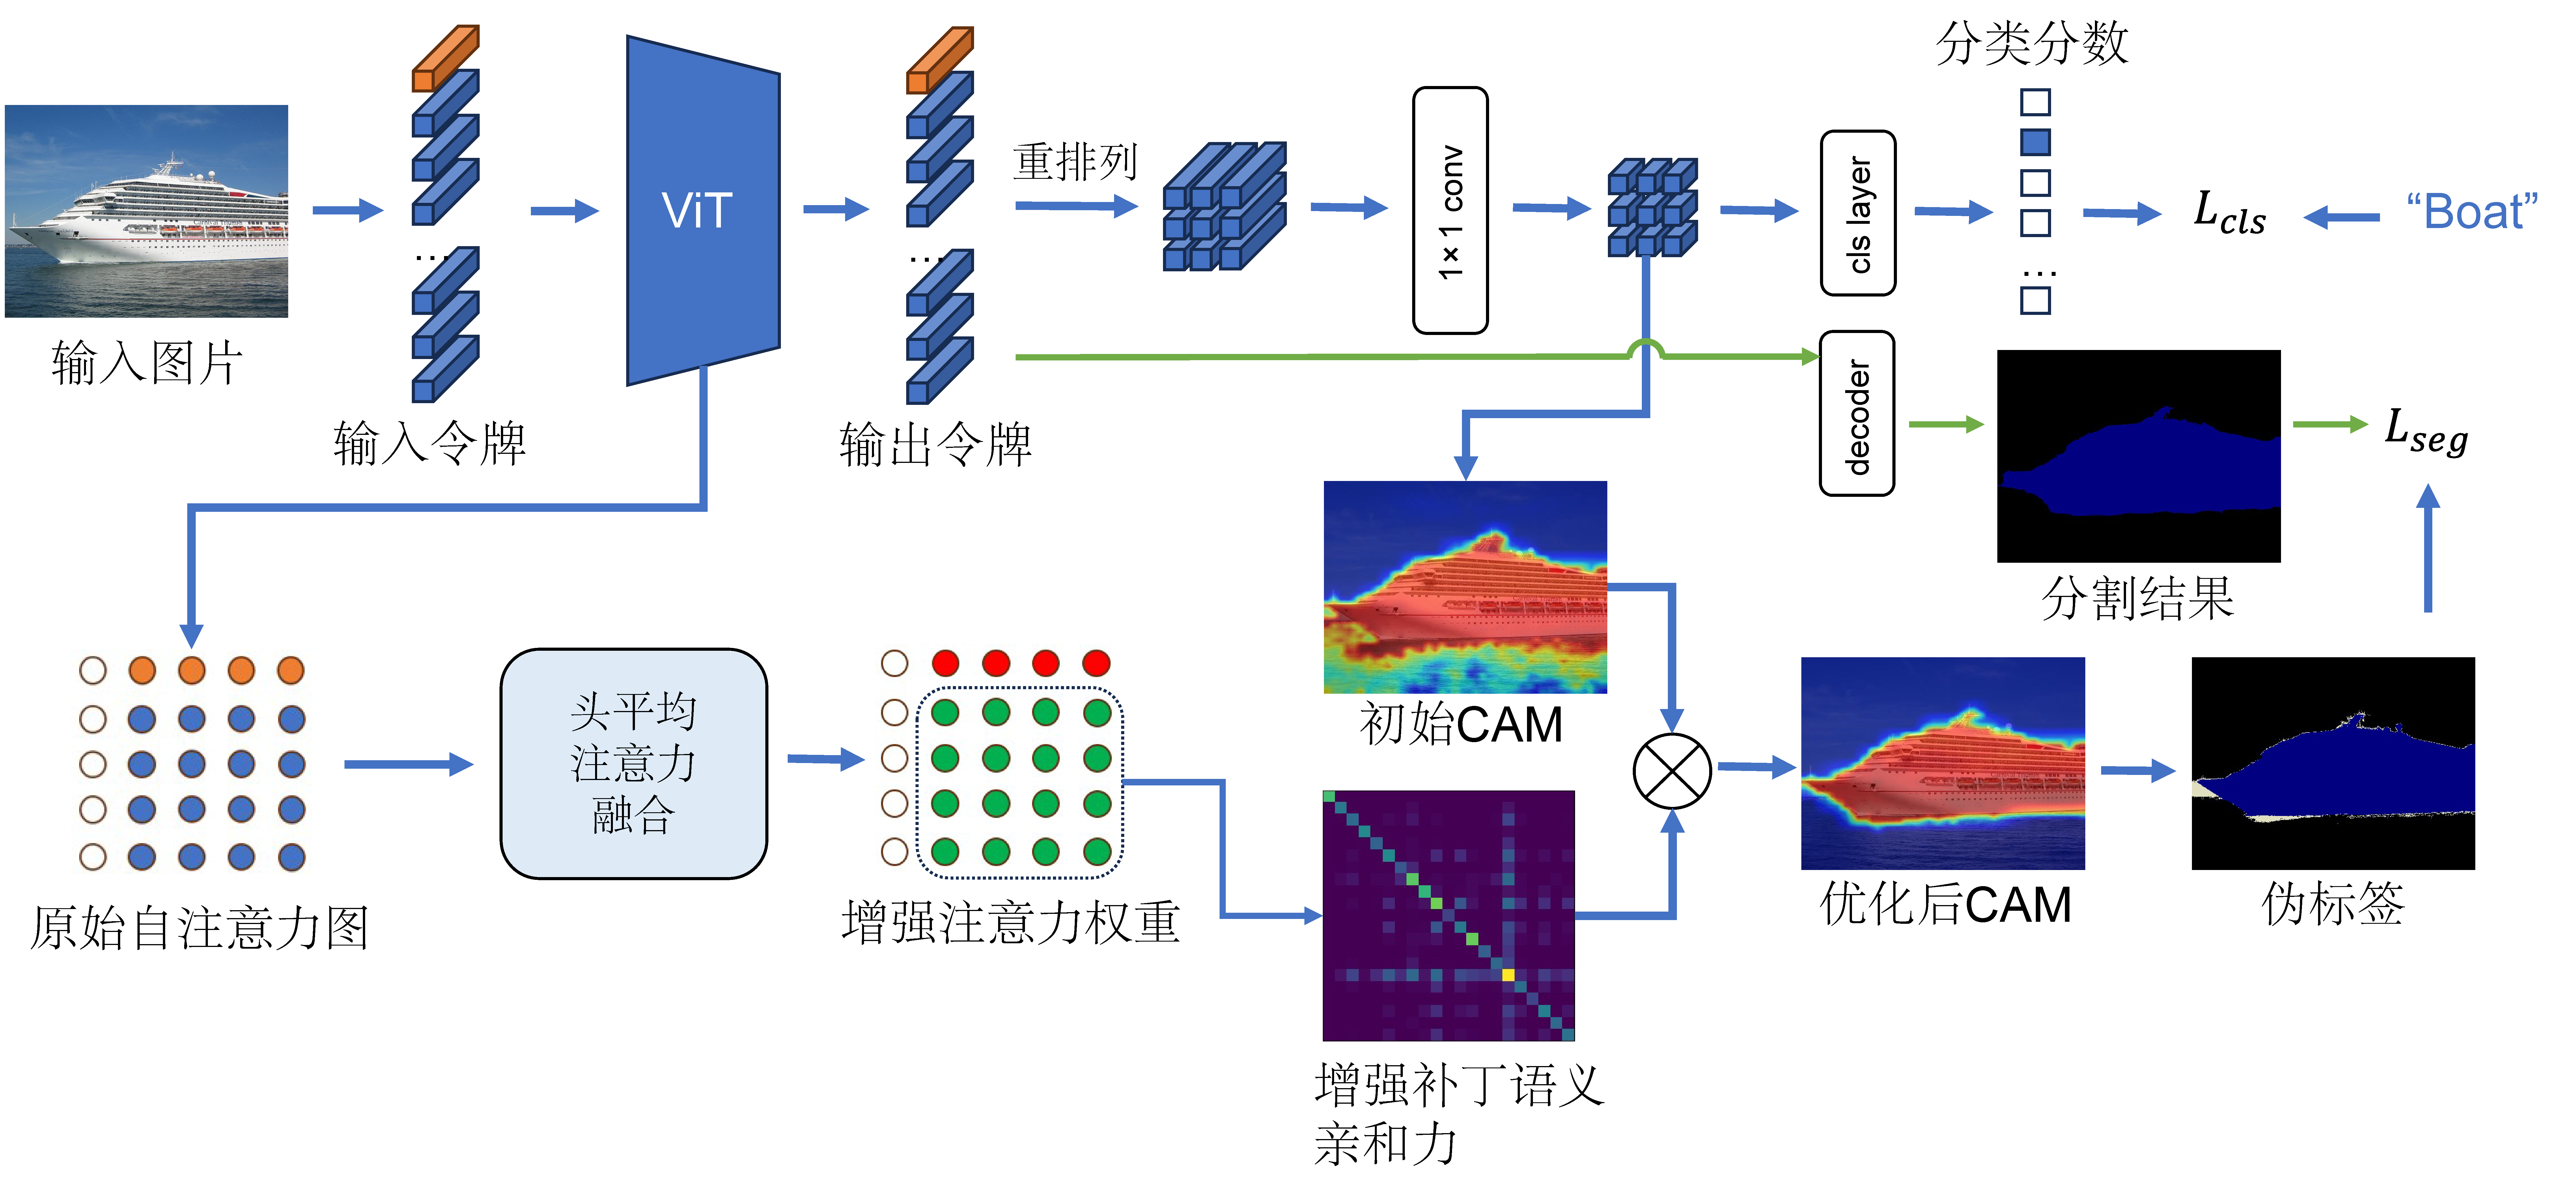
\includegraphics[width=6in]{fig/fig1.pdf}}
    \begin{CJK*}{UTF8}{fs}
        \caption{SS-EPA整体框架。SS-EPA首先将输入图像分成多个补丁,每个补丁线性转换成补丁令牌,并连接一个类别令牌。ViT输出令牌一方面经过重拍列和$1\times 1$卷积生成初始CAM,并由分类层输出分类分数。另一方面经过分割decoder生成语义分割结果。然后从ViT中提取多头自注意力图,并通过HAAF模块进行增强,获取增强补丁语义亲和力。最后通过增强补丁语义亲和力对初始CAM进行优化,并生成伪标签用于监督分割任务。}\label{fig1}
    \end{CJK*}
\end{figure*}

\begin{CJK*}{UTF8}{zhhei}
    \zihao{5}
    \vskip 1mm
    \section{引言}
\end{CJK*}

\begin{CJK*}{UTF8}{fs}
    深度学习推动图像分割显著进步,但依赖精确标注样本,成本高昂。弱监督语义分割(WSSS)技术因此出现,WSSS仅需粗略标注的样本,大幅降低了样本获取的难度。弱监督标注分为边框级标注\cite{39dai2015boxsup,40zhang2021affinity}、涂鸦级标注\cite{41lin2016scribblesup}和图像级标\cite{03ru2023token,12xu2022multi}。其中最难利用的是图像级标注,因为它通常只提供图片的分类标签,包含极少可利用的语义信息,也是多数研究人员最热衷于研究的方法之一。本工作只使用图像级弱标注。

	先前的WSSS方法通常采用多阶段方法,即先训练一个分类网络来生成类激活图Class Activation Map(CAM)\cite{01zhou2016learning},获取类别在图像中的位置信息。然后通过扩展优化CAM生成伪标签,最后利用伪标签全监督地训练语义分割模型。虽然多阶段方法通常可以获得更精准的CAM和更优秀的分割性能,但通常需要分阶段地训练模型和不同的训练策略,耗费大量的计算资源和时间来进行训练和优化,这限制了其在大规模数据集或实时应用中的实用性。通过CNN生成的CAM,存在只激活最显著区域的缺点,原因是CNN感受野有限,对全局信息捕获不完善。Vision Transformer(ViT)\cite{02dosovitskiy2020image}在其它视觉任务中的巨大成功,引起了WSSS领域研究人员的广泛关注\cite{03ru2023token,12xu2022multi,13ru2022learning}。ViT是一种基于 Transformer 架构的视觉模型,它将输入图片划分为小的补丁(patch),并利用Transformer 来建模这些补丁之间的关系。且ViT采用无卷积架构,避免了卷积带来的先验约束,如局部性和平移不变性,使ViT具有更好的可扩展性。基于ViT的WSSS方法首先通过补丁令牌生成粗略的初始CAM,再利用多头自注意力中包含的语义亲和力信息对初始CAM进行优化\cite{12xu2022multi}。然而Transformer中不同深度层的多头自注意力可能关注不同部分,如浅层更关注局部结构、纹理颜色等,深层能捕获更广泛和抽象的视觉语义信息,直接将其与CAM相乘可能会产生错误与误导。且ViT注意力图十分庞大,直接提取所有注意力权重会占据大量计算资源。

	本文提出一种单阶段 WSSS 方法 SS-EPA (Single Stage WSSS with Enhanced Patch Affinity) ,和一种头平均注意力融合增强模块 (Head Average Attention Fusion,HAAF) 。针对先前 CAM 优化多数集中在多阶段方法上的问题,本文提出一种单阶段 WSSS 方法 SS-EPA ,集成了端到端式多头自注意力 CAM 优化方法。 SS-EPA 从 ViT 的自注意力中提取补丁语义亲和力信息,并用于优化初始 CAM 。本文将该端到端的优化方法集成到单阶段 WSSS 方法中,不会影响其完整性和一致性。针对注意力图较为庞大,且不同深度的注意力特性各不相同的问题,本文提出一种头平均注意力融合增强模块 HAAF 。 HAAF 对来自不同层多头自注意力中的语义亲和力进行融合增强,并用于优化从 Transformer 生成的 CAM 。 HAAF 通过对多头自注意力中的各头权重进行平均,聚合不同语义信息,减少不同头重复关注相似区域的冗余信息。随后,通过全局平均池化聚合每个注意力图的全局特征,并将其输入多层感知机,提取更复杂的特征关系。最终获得融合后的增强注意力图,充分考虑了不同层次注意力的重要性。 HAAF 可以去除头重复关注、包含无效信息的冗余问题,显著降低计算资源消耗并提升效率。该方法还能减少每个头对噪声或异常的敏感度,提高模型鲁棒性。

	为了验证本文提出的 SS-EPA 和 HAAF 模块的有效性,本文在 Pascal VOC 2012数据集上评估了SS-EPA的CAM、伪标签和分割结果的性能表现,并与基线方法ToCo\cite{03ru2023token}相比较。对比实验、消融实验以及各种可视化结果表明,本文所提方法可以显著优化生成的CAM,伪标签和分割模型误分类的概率更小,且有更加完整和准确的对象边界。在VOC验证集上与基线相比,伪标签和分割性能分别提升了2.2\%和1.3\%的mIoU分数,充分验证了本文方法的有效性。

    总的来说,本文主要贡献包括以下三个方面:
    \begin{itemize}
        \item 提出了一种名为 SS-EPA 的单阶段 WSSS 方法,集成了端到端式多头自注意力 CAM 优化方法。在不影响单阶段方法的完整性和一致性的前提下,集成了利用补丁语义亲和力信息优化初始 CAM 的方法,使 CAM 更加精细和准确,从而生成更加优质的伪标签用于训练分割模型。
        \item 提出一种头平均注意力融合增强模块(HAAF),来解决语义亲和力信息包含噪声与错误,以及注意力图较为庞大的问题。通过对注意力的不同头的权重做平均,HAAF可去除冗余信息并提高模型鲁棒性,利用多层感知机的交互能力,HAAF可以充分考虑来自不同层注意力的重要性,对包含语义亲和力的自注意力完成简化和增强。
        \item 在 Pascal VOC 2012 数据集上的实验表明,本文方法可以显著优化生成的 CAM ,最终的分割模型性能相比以前的单阶段方法有了实质性的改进,且实现了与一些多阶段方法相当的性能。
    \end{itemize}
\end{CJK*} %添加引言
\begin{CJK*}{UTF8}{zhhei}
    \zihao{5}
    \vskip 1mm
    \section{相关技术}
\end{CJK*}



\begin{CJK*}{UTF8}{zhhei}
    \subsection{图像级弱监督语义分割}
\end{CJK*}

图像级WSSS是所有WSSS方法中挑战性最大的一种。该方法仅依赖于图像的分类标签。与其它形式的弱标注,如涂鸦标注和边框标注相比,图像级标注所提供的信息量更为有限,因此在实现像素级精细分割的任务上难度更高。利用图像级标注的WSSS方法通常生成CAM来获取图像分类时的关注区域,从而捕获特定于类别的定位信息\cite{42ahn2018learning}。但CAM激活的区域通常只会覆盖最明显最具判别力的对象区域,而忽略其它非判别性的区域。一些工作专注于生成高质量CAM,如对抗性擦除方法\cite{04wei2017object},通过擦除最具判别力的对象区域来迫使模型关注其它非判别性的区域,可以一定程度上优化缓解CAM激活不全的问题。还有工作利用子类别探索\cite{05chang2020weakly}、自监督注意力机制\cite{06wang2020self}和多图像语义信息\cite{07li2021group}来获得更精准的CAM。最近也有工作\cite{08xie2022clims,09lin2023clip}利用了CLIP\cite{10radford2021learning}模型,利用CLIP对图像和文本强大的上下文理解能力抑制背景像素的激活,更专注于前景区域。然而这些方法大多集中于多阶段WSSS方法,且需要分阶段地训练模型和不同的训练策略,多个阶段间的复杂交互较为繁琐。本文提出的单阶段WSSS方法SS-EPA,集成了端到端式多头自注意力CAM优化方法,减少了流程复杂性。 

\vspace{2mm}

\begin{figure*}[htbp]
    \centerline{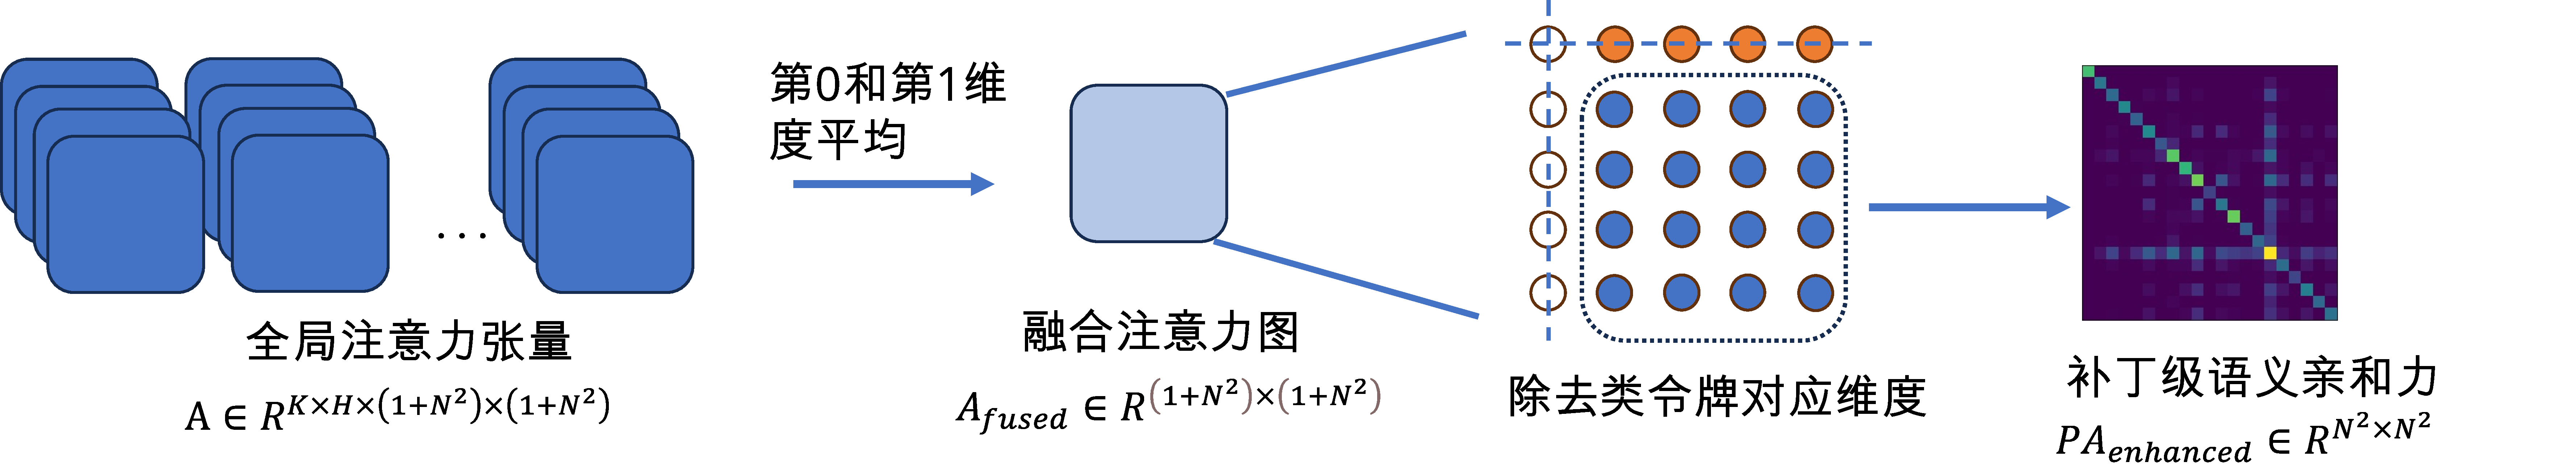
\includegraphics[width=6in]{fig/fig2.pdf}}
    \begin{CJK*}{UTF8}{fs}
        \caption{补丁语义亲和力获取流程图}\label{fig2}
    \end{CJK*}
\end{figure*}

\begin{CJK*}{UTF8}{zhhei}
    \subsection{弱监督语义分割中的ViT}
\end{CJK*}

先前的WSSS方法大多建立在CNN网络之上,存在只激活最显著区域的缺点。ViT\cite{02dosovitskiy2020image}凭借其强大的全局上下文建模能力,在WSSS任务中取得成功。TS-CAM\cite{11gao2021ts}提出借助ViT和多头自注意力的特性生成CAM,来充分利用ViT的长距离建模能力。MCTformer\cite{12xu2022multi}强调了ViT中类令牌的重要性,通过嵌入多个类令牌并强制它们学习不同类的激活图,并利用特定类别的注意力图优化CAM。AFA\cite{13ru2022learning}通过额外的模块学习多头自注意力中的语义亲和力,改善了CAM的覆盖区域,缓解了CAM难以捕捉完整的目标区域的问题。ToCo\cite{03ru2023token}通过利用ViT中间层的伪标记关系来监督最终的补丁标记,从而解决ViT的过度平滑问题。然而,先前的方法通常利用ViT中的语义亲和力优化CAM,对计算资源要求较高,且直接利用可能会给CAM带来错误和误导。且ViT中多头注意力的设计目的是为了捕捉不同依赖关系,但实践中一些注意力头往往会关注相似的区域或信息,导致不同头之间存在相似性,产生冗余。本文提出的头平均注意力融合增强模块(HAAF)通过多头平均化去除上述冗余信息,淡化可能捕捉到的噪声或者无效的注意力模式,减少单个头对特定噪声的敏感度,提高模型的鲁棒性。 %添加相关工作
\begin{CJK*}{UTF8}{zhhei}
    \zihao{5}
    \vskip 1mm
    \section{方法}
\end{CJK*}

\begin{CJK*}{UTF8}{zhhei}
    \subsection{概述}
\end{CJK*}

本节首先介绍了 SS-EPA 的整体框架, SS-PEA 是一种改进的单阶段 WSSS 方法,集成了端到端式多头自注意力 CAM 优化方法。 SS-EPA 首先通过 ViT 对输入图片分类,并生成初始 CAM 。然后结合补丁语义亲和力优化 CAM ,并生成伪标签用于监督分割任务,实现图像分类和语义分割的联合学习。如图\ref{fig1}所示, SS-EPA 是单阶段 WSSS 方法,集成了端到端式多头自注意力 CAM 优化方法,相比传统多阶段方法简化了流程。本文提出了头平均注意力融合增强模块 (HAAF) ,来去除不同头重复关注相似区域的冗余信息,并提高模型鲁棒性。解决了多头自注意力图较为庞大,且直接利用语义亲和力会带来噪声与错误的问题\cite{12xu2022multi}。

% \begin{figure*}[htbp]
%     \centerline{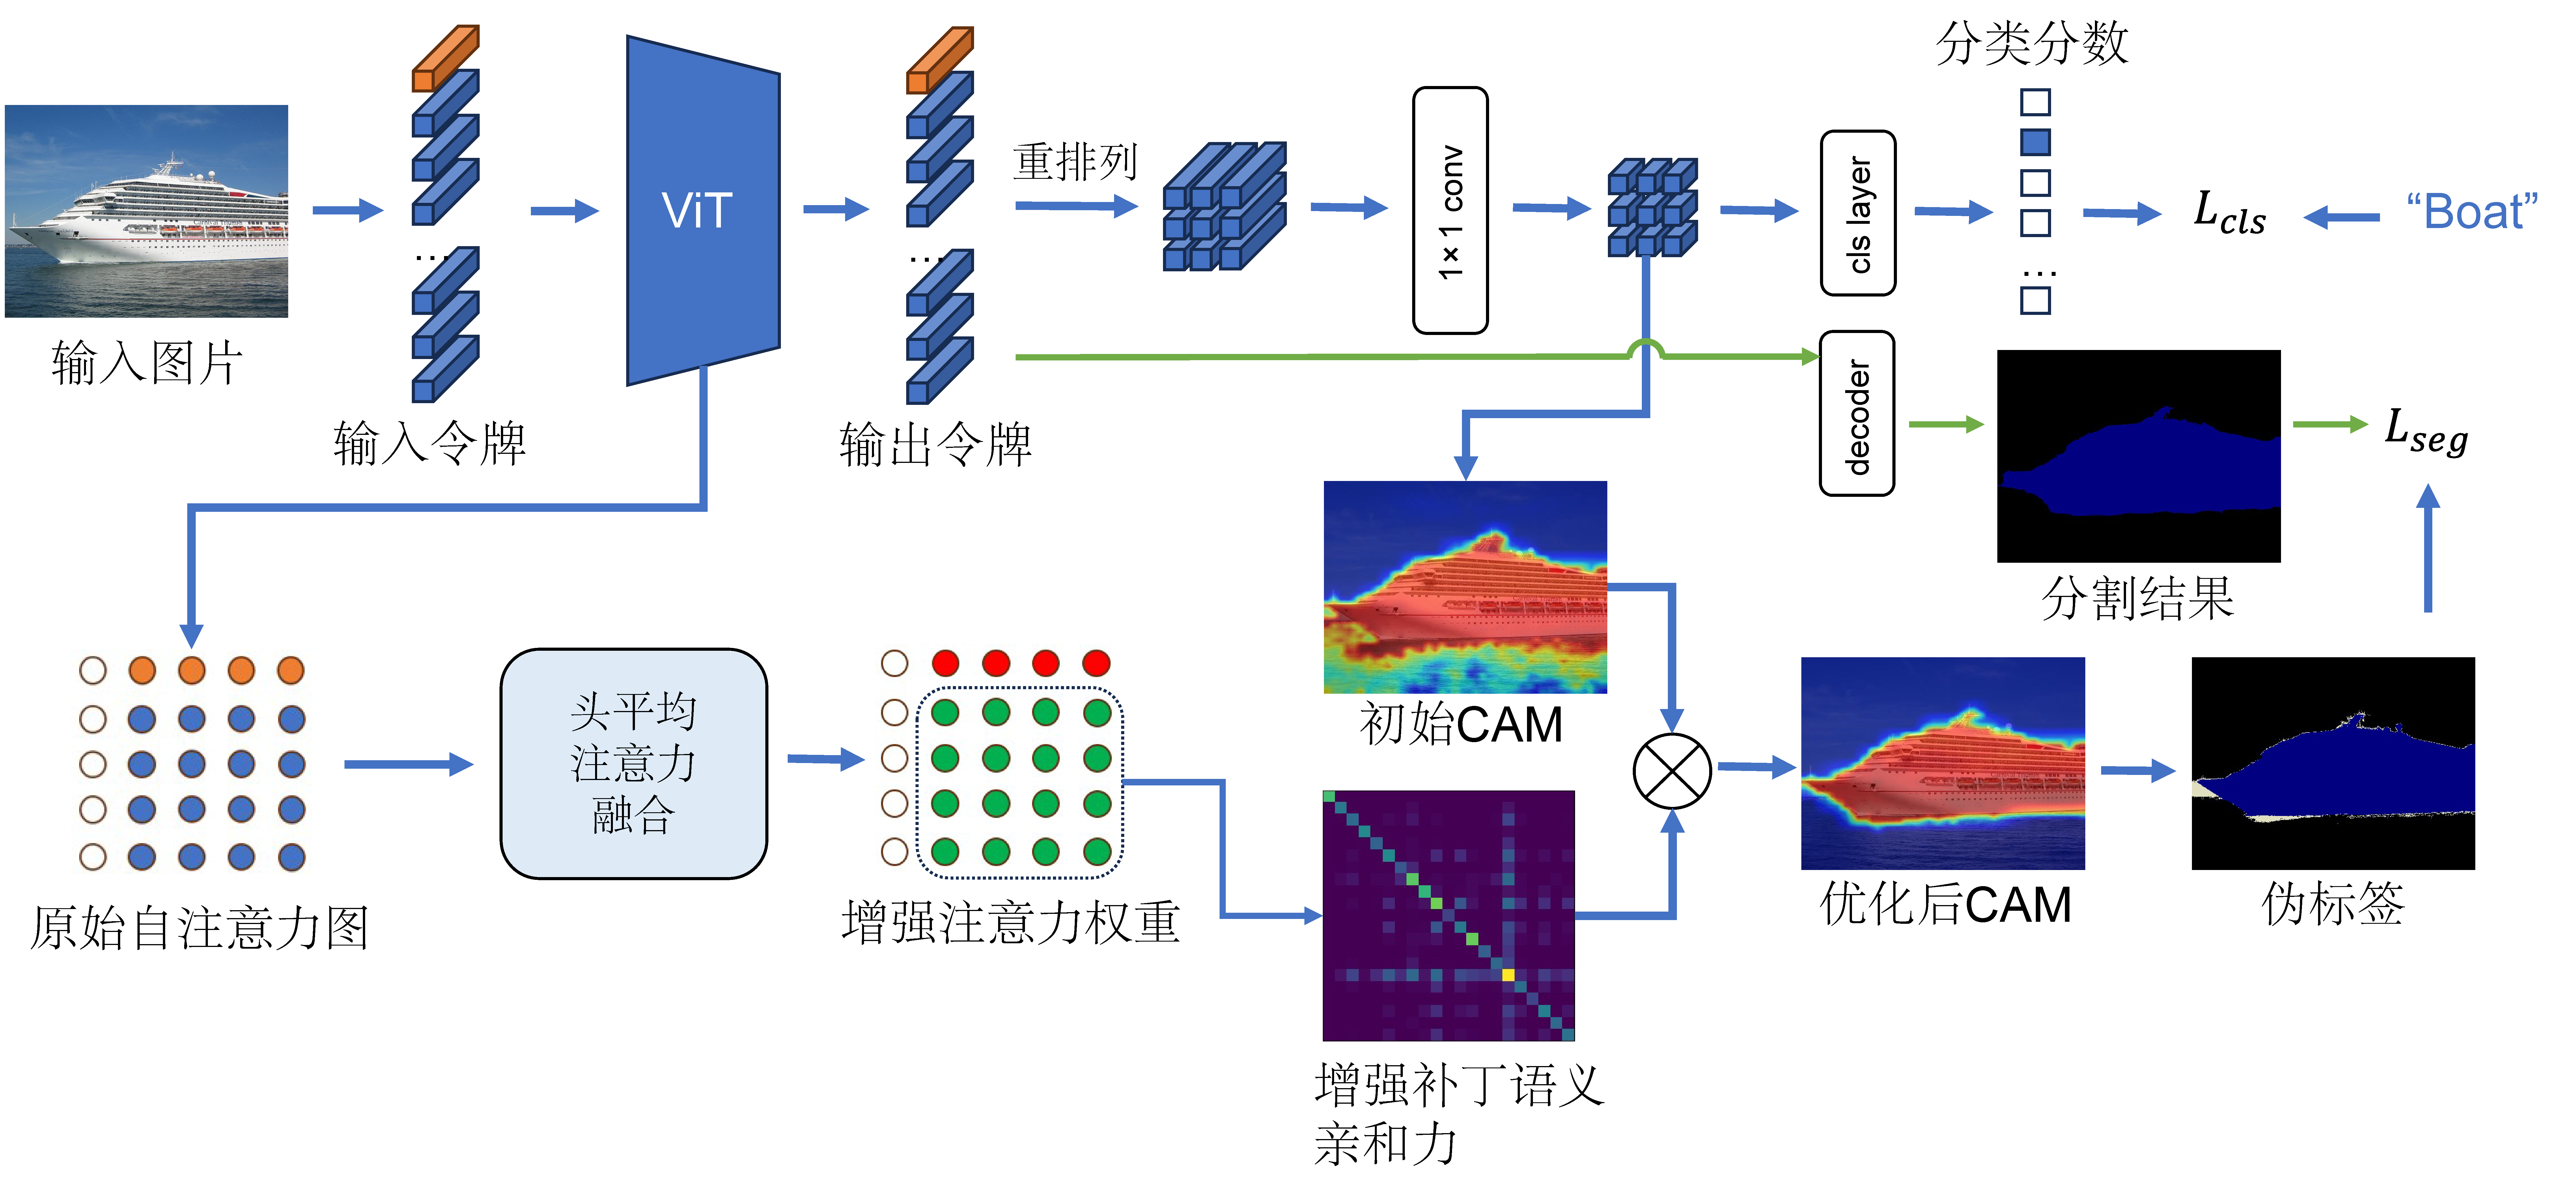
\includegraphics[width=6in]{fig/fig1.pdf}}
%     \begin{CJK*}{UTF8}{fs}
%         \caption{SS-EPA整体框架。SS-EPA首先将输入图像分成多个补丁,每个补丁线性转换成补丁令牌,并连接一个类别令牌。ViT输出令牌一方面经过重拍列和$1\times 1$卷积生成初始CAM,并由分类层输出分类分数。另一方面经过分割decoder生成语义分割结果。然后从ViT中提取多头自注意力图,并通过HAAF模块进行增强,获取增强补丁语义亲和力。最后通过增强补丁语义亲和力对初始CAM进行优化,并生成伪标签用于监督分割任务。}\label{fig1}
%     \end{CJK*}
% \end{figure*}

\vspace{2mm}

\begin{CJK*}{UTF8}{zhhei}
    \subsection{SS-EPA框架}\label{section3.2}
\end{CJK*}





SS-EPA首先将输入图片拆分为 $N\times N$ 个补丁,并通过线性转换为补丁令牌序列 $T_{\text{patch}}\in R^{N^2\times D}$,其中D是嵌入维度。
生成一个维度同样为D的类令牌 $T_{\text{cls}}\in R^{1\times D}$,将类令牌与补丁令牌链接,并添加位置编码构成ViT编码器的输入令牌序列 $T_{\text{input}}\in R^{(1+N^2)\times D}$。
ViT backbone具有$K$个Transformer编码层,每个编码层包含一个多头自注意力和一个多层感知机,以及分别用于两个子层前的层归一化。
ViT编码器接收输入令牌序列$T_{\text{input}}^i,i=(1,2,…,K)$,并输出令牌序列$T_{\text{out}}^i\in R^{(1+N^2)\times D},i=(1,2,…,K)$。
最后一层Transformer编码层的输出令牌序列$T_{\text{out}}^K\in R^{(1+N^2)\times D}$,去除类令牌对应维度并重排列可得补丁令牌序列$T_{\text{out\_patch}}\in R^{N\times N\times D}$,并执行$1\times 1$卷积操作将令牌维度变为物体类别数量,公式如下:

\begin{equation}
    \text{CAM}=\text{conv}_{1\times 1} (T_\text{out\_patch})
\end{equation}
其中,$\text{conv}_{1\times 1}$的输入通道为D,输出通道为物体类别数$C$,卷积核大小为$1\times 1$。通过上式可获得来自补丁令牌的初始类激活图$\text{CAM}\in R^{N\times N\times C}$。参照\cite{13ru2022learning}的方法,通过一个全局最大池化层(Global Max Pooling)来聚合补丁令牌$T_{\text{out\_patch}}$信息,然后通过全连接层来计算分类分数cls\_score,分类损失函数使用多标签软边距损失(Multi Label Soft Margin Loss)作为损失函数$L_{cls}$,公式如下:
\begin{equation}
    \begin{aligned}
        L_\text{cls}(x,y) = - \frac{1}{C}&\sum_{i=1}^C [y\log(\sigma (x)) \\
        &+(1-y)\log(1-\sigma (x))]
    \end{aligned}
\end{equation}
其中$x$,$y$分别是模型预测分数与真值标签,$\sigma(x)$表示Sigmoid函数的输出,即:
\begin{equation}
    \sigma(x) = \frac{1}{1+e^{-x}}
\end{equation}

ViT backbone使用的是标准的 Transformer 多头自注意力,首先将输入令牌归一化,并通过全连接层将其转换为一个查询$Q\in R^{(1+N^2)\times D}$和一组键值$K\in R^{(1+N^2)\times D}$、$V\times R^{(1+N^2)\times D}$,注意力计算采用\cite{14vaswani2017attention}中的缩放点积注意力(Scaled Dot-Product Attention),计算公式如下:

\begin{equation}
    \text{Attn}(Q,K,V)=\left(\text{Softmax}\frac{QK^T}{\sqrt{D}}\right)V
\end{equation}
从中可以提取多头自注意力图$A_{map}=QK^T$,其中$A_{\text{map}}^i\in R^{H\times (1+N^2)\times (1+N^2)} ,i=1,\cdots,K$,$H$为多头自注意力头的个数。此操作不会带来任何额外的计算资源消耗,因为多头自注意力权重是Transformer在计算时产生的副产物。然后在第$0$个维度上进行concatenate操作将$K$层注意力图串联起来,获得全局注意力张量$A\in R^{K\times H\times (1+N^2)\times (1+N^2)}$,该注意力张量十分庞大,在\ref{section3.3_HAAF}节中将讨论如何减小计算资源占用。

% \begin{figure*}[htbp]
%     \centerline{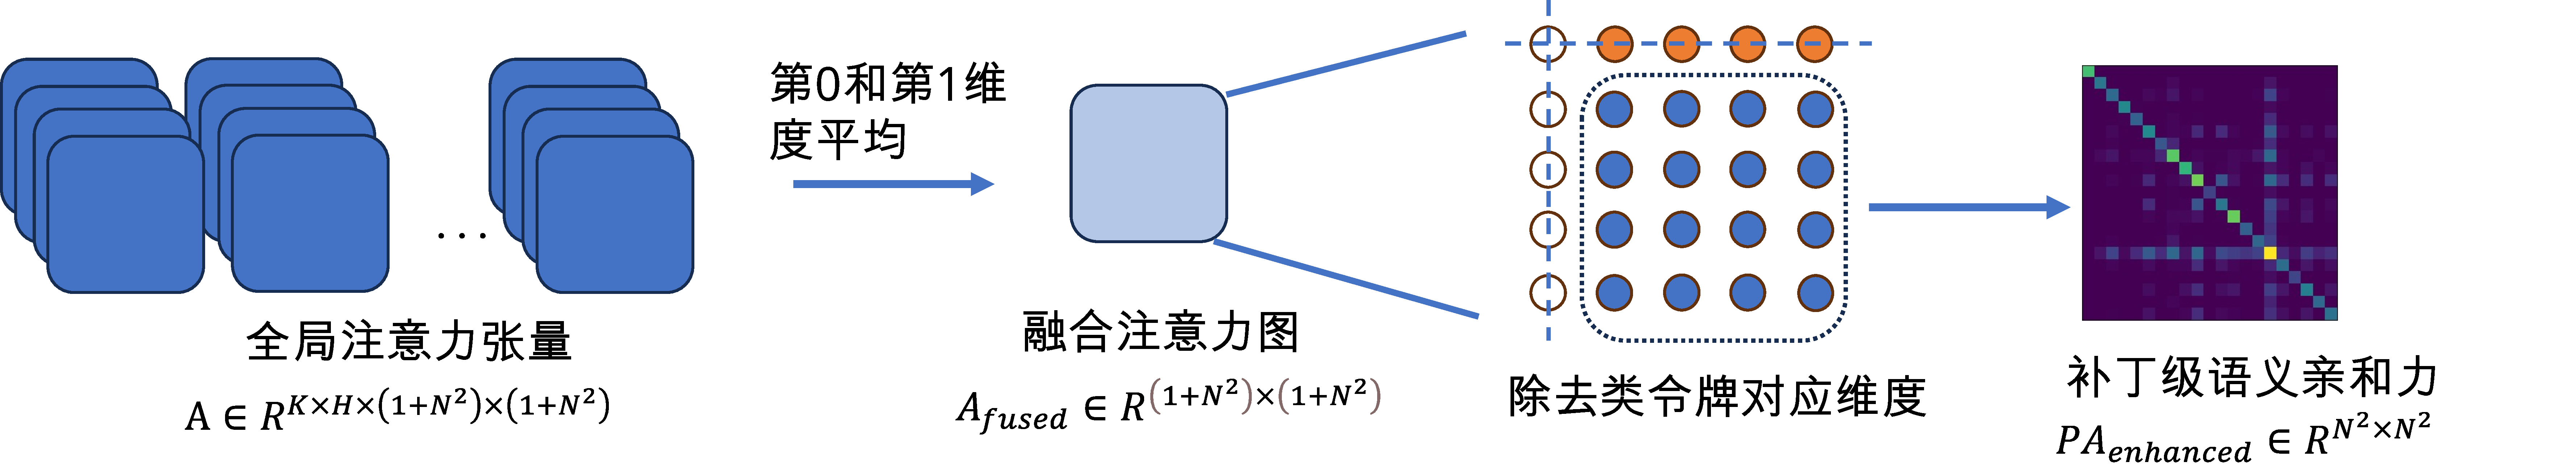
\includegraphics[width=6in]{fig/fig2.pdf}}
%     \begin{CJK*}{UTF8}{fs}
%         \caption{补丁语义亲和力获取流程图}\label{fig2}
%     \end{CJK*}
% \end{figure*}

全局注意力张量$A$中蕴含了补丁语义亲和力信息,将注意力图$A$在第$0$和第$1$个维度上进行平均来聚合来自不同层和不同头的注意力信息,得到$A_{\text{fused}}\in R^{(1+N^2)\times (1+N^2)}$,除去其中类令牌对应的维度,如图\ref{fig2}所示,剩下的注意力权重可作为补丁级语义亲和力$\text{PatchAffinity}\in R^{N^2 \times N^2}$。由于从补丁令牌生成的初始类激活图CAM存在大量噪声与错误,所以需要补丁级语义亲和力对其进行优化,优化公式如下:

\begin{equation}
    \text{CAM}_{\text{refined}}=\text{PatchAffinity}\times \text{CAM}
\end{equation}

通过上式可获得通过原始补丁语义亲和力优化后的类激活图$\text{CAM}_\text{refined}\in R^{N\times N\times C}$,相比初始CAM对目标的覆盖性更好,错误激活区域更少,且可以激活更多目标区域。


\vspace{2mm}


\begin{CJK*}{UTF8}{zhhei}
    \subsection{头平均注意力融合增强模块(HAAF)}
    \label{section3.3_HAAF}
\end{CJK*}

鉴于 Transformer 中不同深度的层的多头自注意力可能关注不同部分,如浅层更关注局部结构、纹理颜色等,深层能捕获更广泛和抽象的视觉语义信息,所以不能简单地将来自不同层的多头自注意力平均来聚合语义信息。
且一个标准ViT backbone(vit\_base\_patch16\_224)的多头自注意力图十分庞大(batchsize为2时,显存占用超过12GB),对计算资源要求较高。
本文提出头平均注意力融合增强模块(HAAF)来解决上述问题,如图\ref{fig3}所示。

\begin{figure}[htbp]
    \centerline{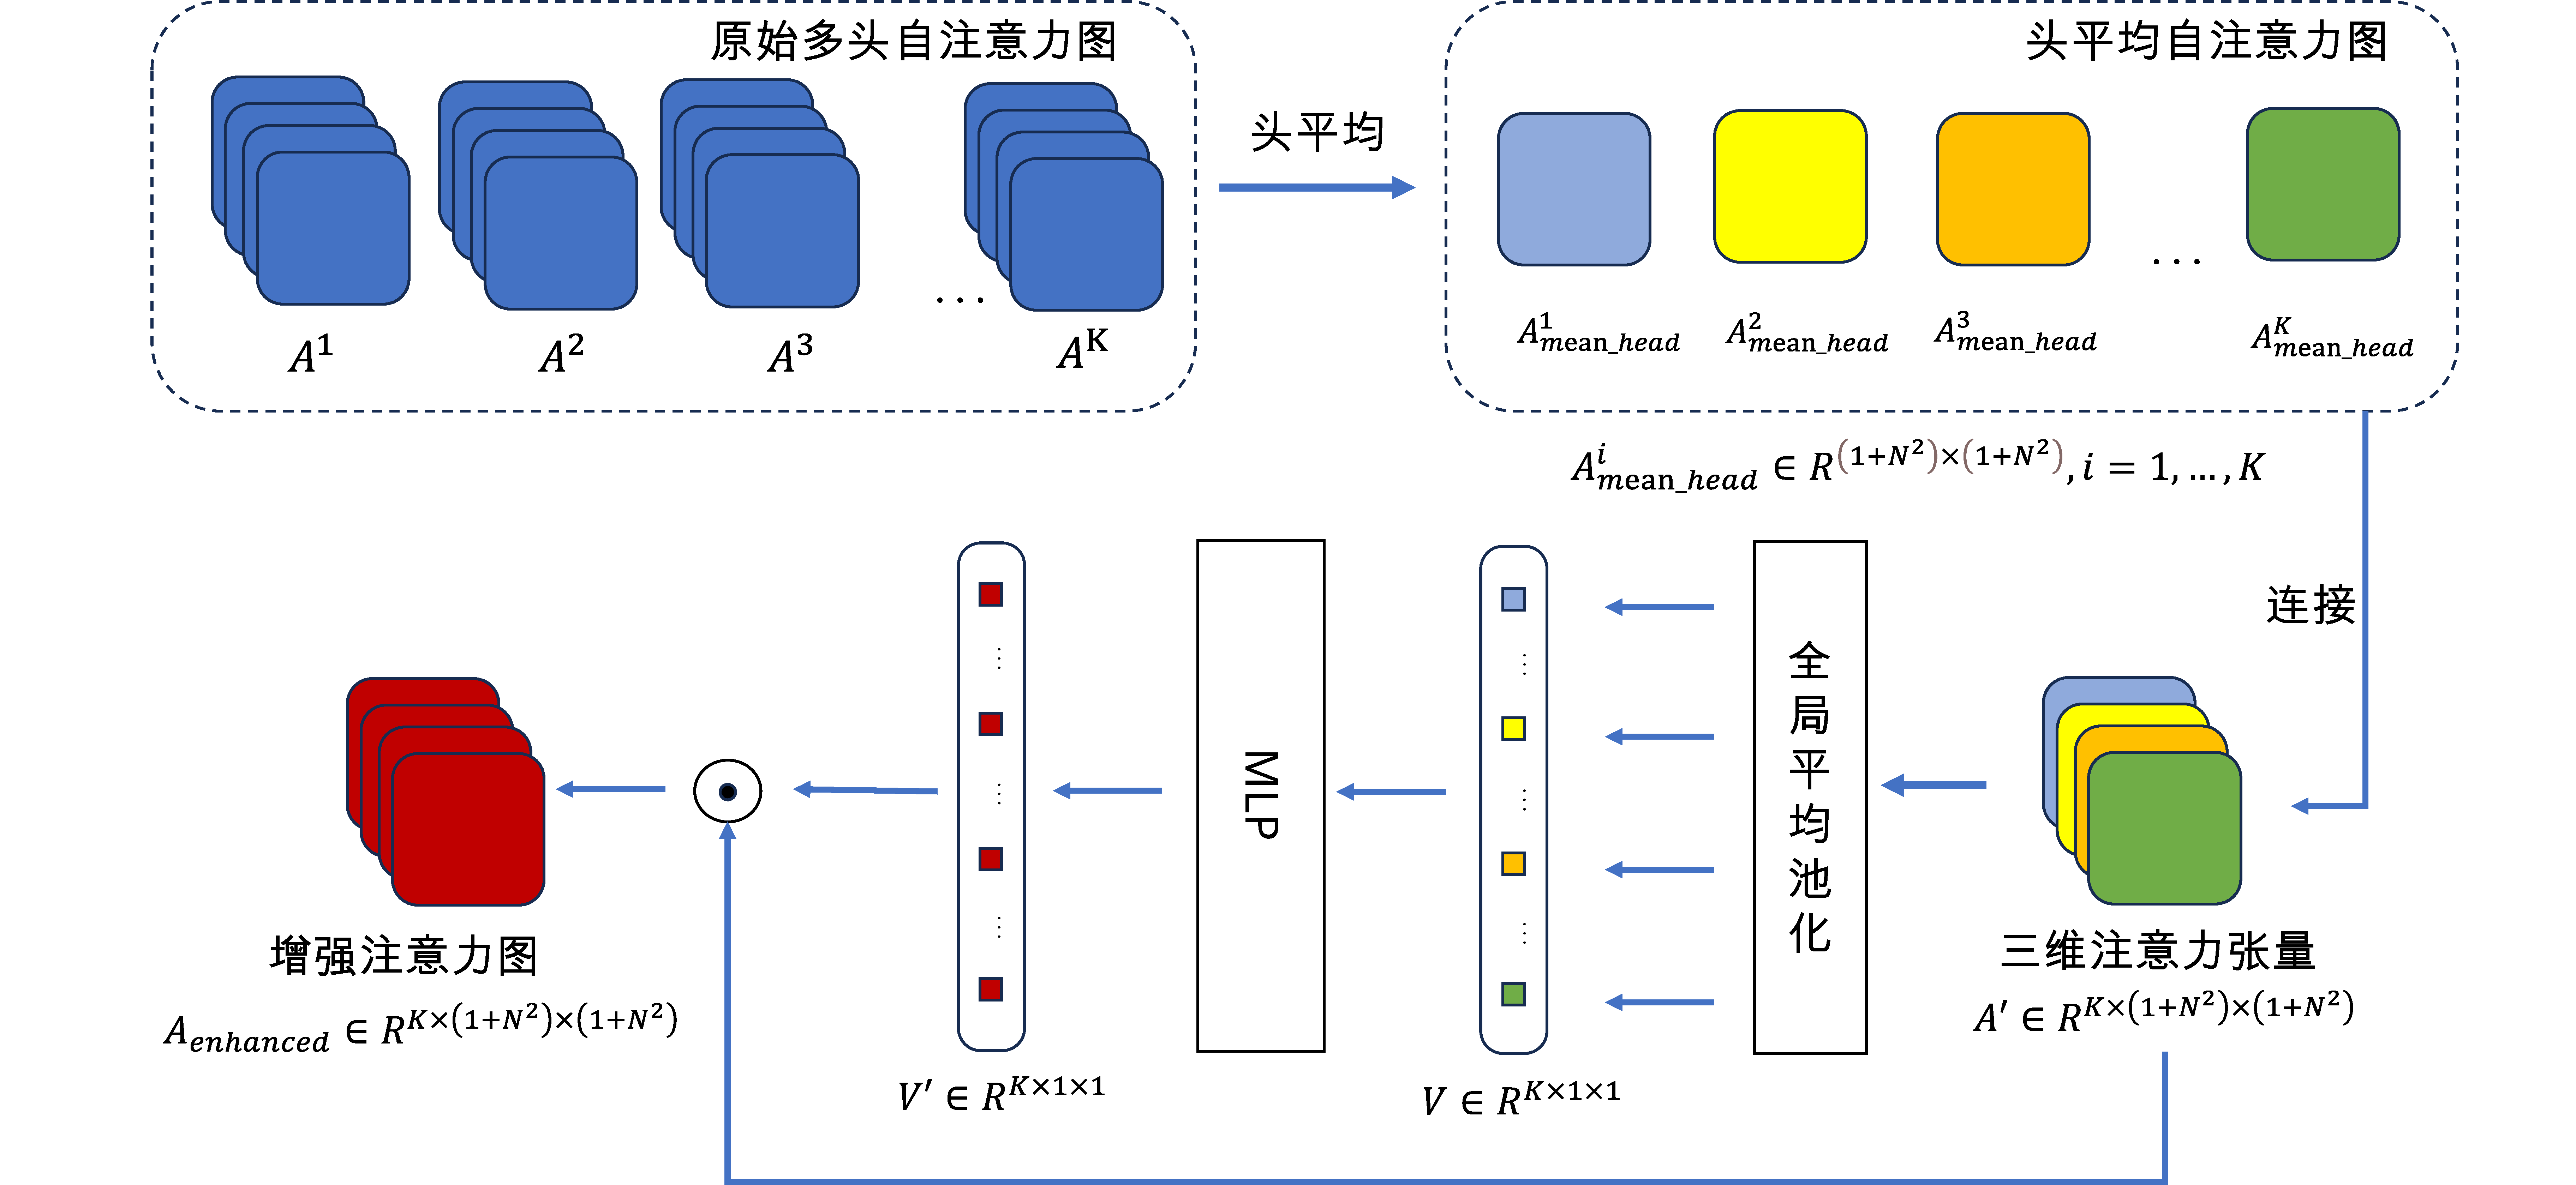
\includegraphics[width=3.15in]{fig/fig3.pdf}}
    \begin{CJK*}{UTF8}{fs}
        \caption{HAAF结构图}\label{fig3}
    \end{CJK*}
\end{figure}

\begin{figure*}[t]
    \centerline{
\includegraphics[width=6in]{fig/fig4.pdf}}
    \begin{CJK*}{UTF8}{fs}
        \caption{增强补丁语义亲和力获取流程图}\label{fig4}
    \end{CJK*}
\end{figure*}

对于\ref{section3.2}节中从backbone中提取的多头自注意力图$A_\text{map}^i\in R^{H\times (1+N^2)\times (1+N^2)},i=1,…,K$,HAAF首先采用头平均操作去除维度$H$,有助于去除冗余信息并减少$H$倍的显存占用,得到$A_\text{mean\_head}^i\in R^{(1+N^2)\times (1+N^2)},i=1,…,K$。
然后在第$0$个维度上进行concatenate操作将$K$层注意力图串联起来,获得全局注意力张量$A'\in R^(K\times (1+N^2)\times (1+N^2) )$。全局平均池化通过平滑特征表示和增强泛化能力,相较于全局最大池化,在减少噪声和防止过拟合方面更具优势。
所以本文通过全局平均池化聚合K层注意力图的全局特征,得到聚合后的长度为$K$的特征向量$V\in R^{K\times 1\times 1}$,并将特征向量输入多层感知机中相互作用,提取更复杂的特征相互关系,多层感知机输出相同形状的特征向量$V'\in R^(K\times 1\times 1)$。获得多层感知机输出的特征向量$V'$后,将全局注意力张量$A'$与特征向量$V'$结合,公式如下:
\begin{equation}
    A'_\text{enhanced} = A' \odot V'
\end{equation}
其中$\odot$表示逐元素相乘符号。
通过上式可获得充分考虑了不同层注意力重要性的增强注意力图$A_\text{enhanced}'\in R^{K\times (1+N^2)\times (1+N^2)}$。经过头平均后的注意力图更加稳定,不易受到单个注意力头学习偏差的影响。



% \begin{figure*}[htbp]
%     \centerline{
\includegraphics[width=6in]{fig/fig4.pdf}}
%     \begin{CJK*}{UTF8}{fs}
%         \caption{增强补丁语义亲和力获取流程图}\label{fig4}
%     \end{CJK*}
% \end{figure*}

图\ref{fig4}展示了不同层增强注意力图的融合过程,对增强注意力图$A_\text{enhanced}'$在第$0$个维度$K$上进行平均操作,可得到融合增强注意力$A_\text{fused}'\in R^{(1+N^2)\times (1+N^2)}$。
除去其中类令牌对应的维度,剩下的增强注意力权重可作为增强后的补丁级语义亲和力$\text{PA}_\text{enhanced}\in R^{N^2\times N^2}$,如图\ref{fig4}所示。通过HAAF增强后的补丁语义亲和力$\text{PA}_\text{enhanced}$相比增强前减少了噪声与错误,并且充分考虑了不同层注意力的重要性。通过特征向量$V'$对每层注意力进行加权。最后利用$\text{PA}_\text{enhanced}$对CAM优化,过程与3.2节介绍的CAM优化过程类似,优化公式如下:

\begin{equation}
\text{CAM}'_\text{refined} = \text{PA}_\text{enhanced} \times CAM
\end{equation}
其中$\text{CAM}$是来自补丁令牌的初始类激活图$\text{CAM}\in R^{N\times N\times C}$,通过上式可获得通过增强补丁语义亲和力优化后的类激活图$\text{CAM}_\text{refined}'\in R^(N\times N\times C)$。$\text{CAM}_\text{refined}'$相比直接利用语义亲和力优化的$\text{CAM}_\text{refined}$,拥有更全面的激活区域和更精细的对象边界,且有更高的鲁棒性。

\vspace{2mm}
\begin{CJK*}{UTF8}{zhhei}
    \subsection{模型训练与损失函数}
\end{CJK*}

如图\ref{fig1}所示,使用多标签软边缘损失作为分类损失$L_\text{cls}$,使用交叉熵损失作为分割损失$L_\text{seg}$。参照基线方法ToCo[3],本文使用了辅助分类损失$L_\text{m\_cls}$,以及令牌对比损失$L_\text{ptc}$和$L_\text{ctc}$。此外,为了进一步提高性能,还按照先前的方法\cite{13ru2022learning,15tang2018regularized,16zhang2021dynamic,17zhang2020reliability},采用了正则化损失$L_\text{reg}$,所以SS-EPA的损失最终定义如下:

\begin{equation}
    \begin{aligned}
        L=&L_\text{cls}+\lambda_1 L_\text{seg}+\lambda_2 L_\text{m\_cls}\\
        &+\lambda_3 L_\text{ptc}+ \lambda_4 L_\text{ctc}+ \lambda_5 L_\text{reg}
    \label{equation_8}
    \end{aligned}
\end{equation}
其中,超参数$\lambda_i,i=1,2,\cdots,5$用于平衡不同损失的权重。
%添加方法论
\begin{CJK*}{UTF8}{zhhei}
    \zihao{5}
    \vskip 1mm
    \section{实验}
\end{CJK*}


\begin{CJK*}{UTF8}{zhhei}
    \subsection{实验设置}
\end{CJK*}

\begin{CJK*}{UTF8}{zhhei}
    \subsubsection{数据集}
\end{CJK*}
本文在Pascal VOC 2012\cite{18everingham2010pascal}数据集上评估所提方法。Pascal VOC 2012包含20个前景类别和1个背景类别。它有三个子集:训练集(train)、验证集(val)和测试集(test),分别包含1464、1449 和 1456张图片。按照先前方法\cite{06wang2020self,12xu2022multi,13ru2022learning,03ru2023token}的常用做法,本文进一步利用SBD数据集将VOC训练集图片数量扩充至10582。在训练过程中,本文严格只使用图像级分类标签用于监督模型训练。

\begin{CJK*}{UTF8}{zhhei}
    \subsubsection{评估指标}
\end{CJK*}
与先前方法一样,本文使用平均交并比(mean Intersection over Union,mIoU),作为CAM质量、伪标签质量以及语义分割模型性能的评估指标。本文方法在Pascal VOC测试集上的评估结果由官方在线评估服务器给出。

\begin{CJK*}{UTF8}{zhhei}
    \subsubsection{实现细节}
\end{CJK*}

\begin{figure*}[t]
    \centerline{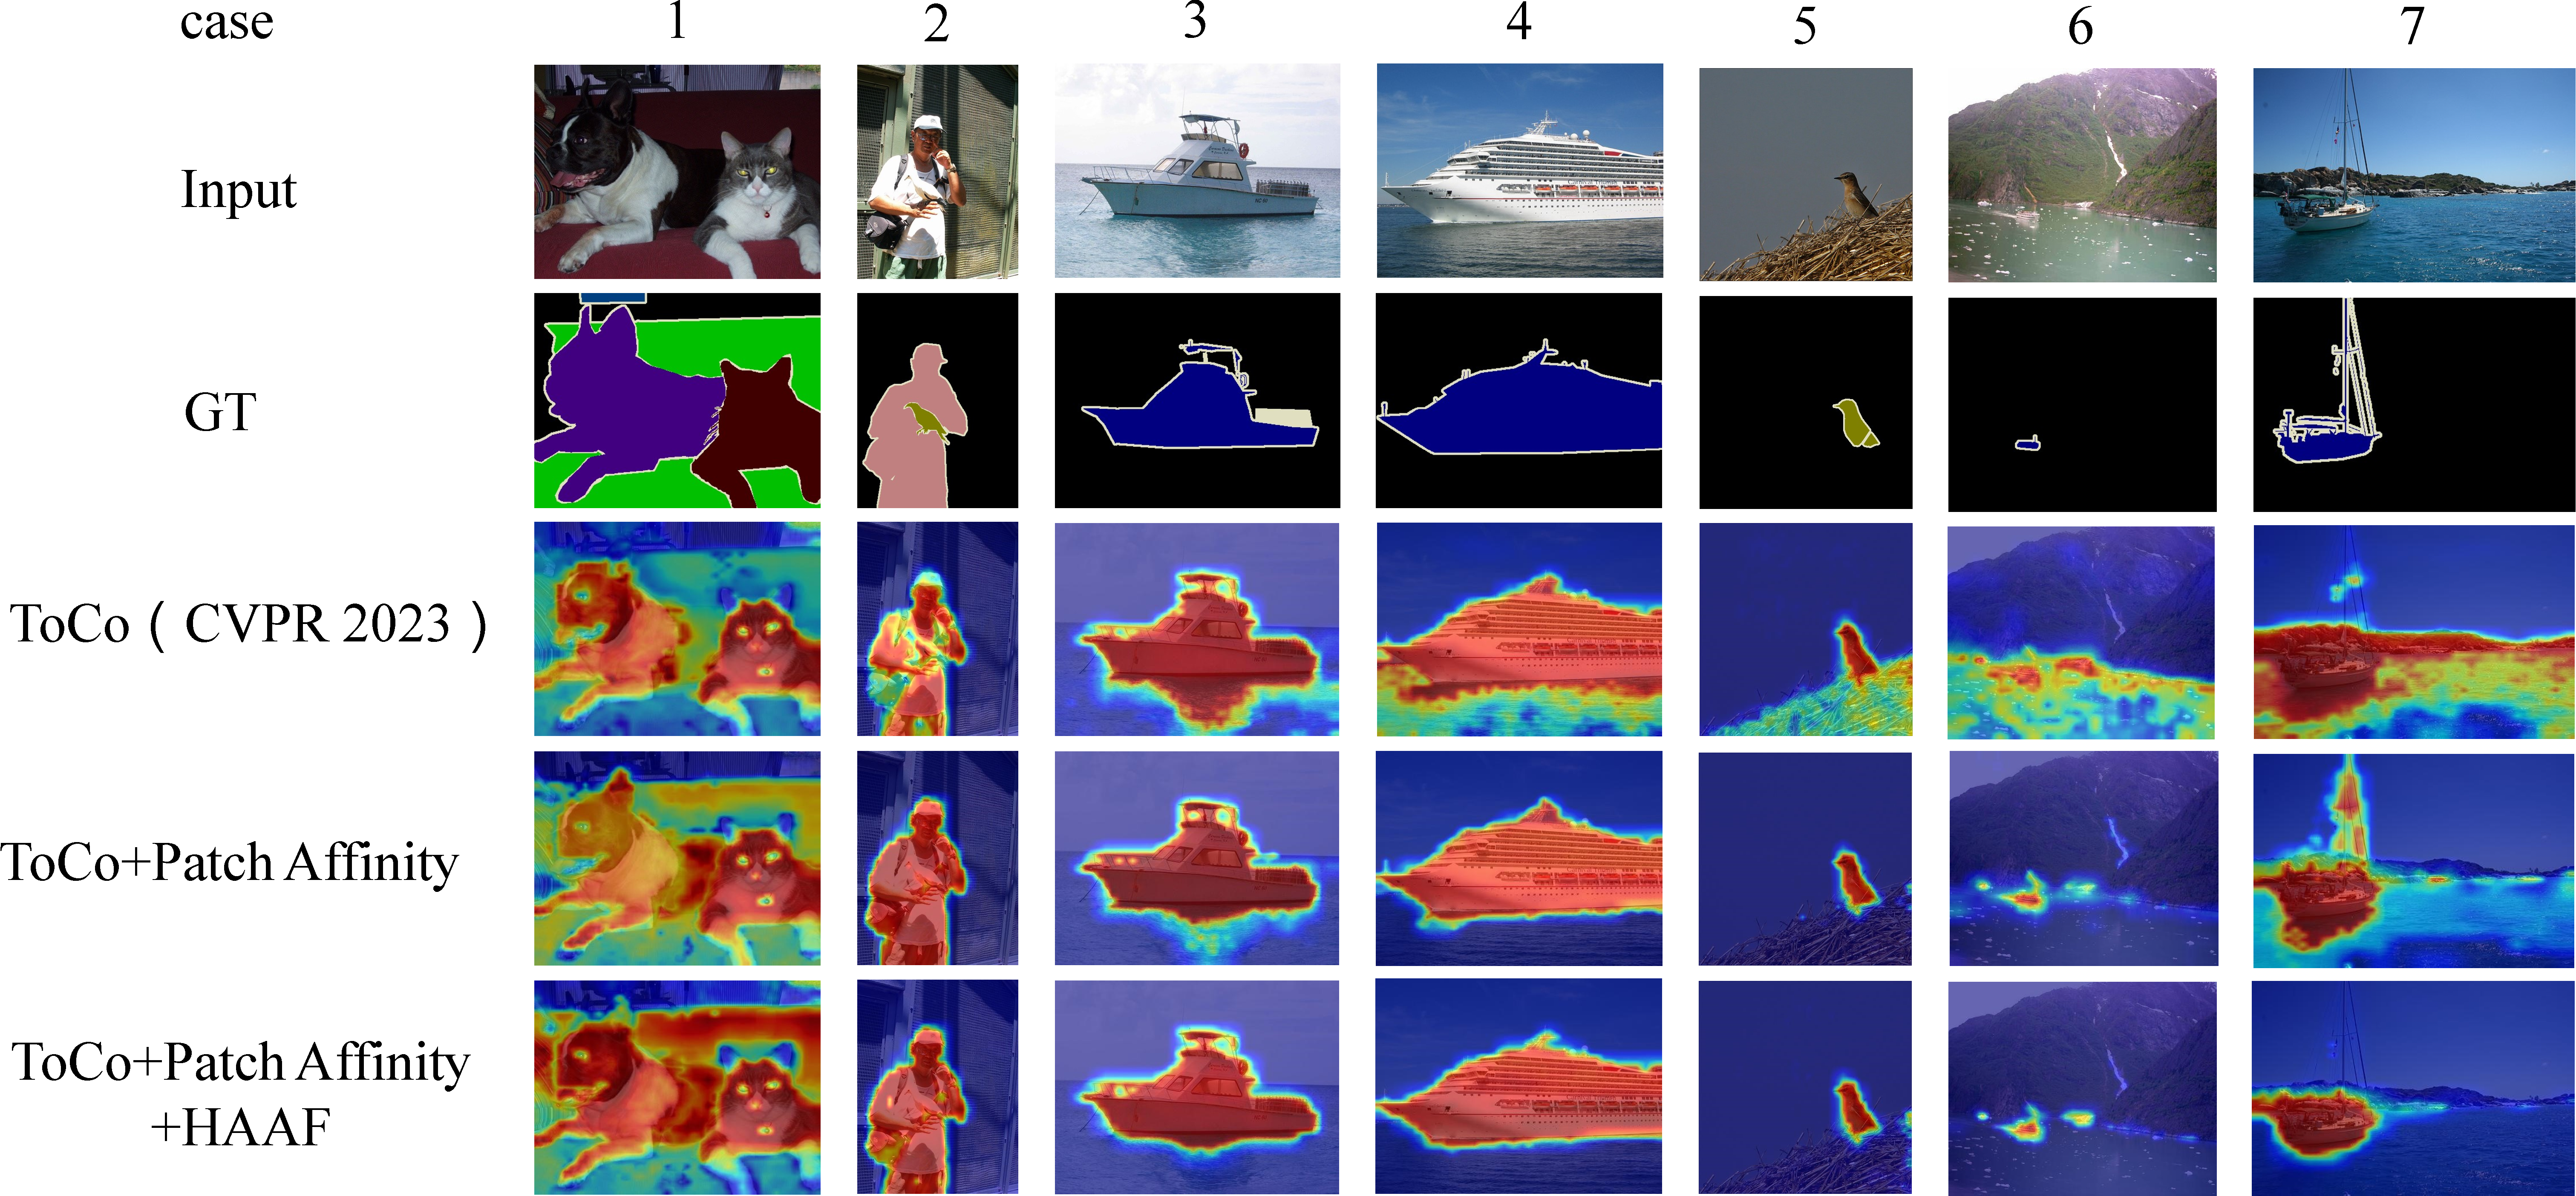
\includegraphics[width=6in]{fig/fig5.pdf}}
    \begin{CJK*}{UTF8}{fs}
        \caption{生成CAM可视化结果,从上到下依次为输入图片(input),真值标签(GT),ToCo生成CAM,SS-EPA生成CAM(不使用HAAF),SS-EPA生成CAM(使用HAAF)。红框部分为显著提升区域。}\label{fig5}
    \end{CJK*}
\end{figure*}

本文利用在 ImageNet 数据集\cite{19deng2009imagenet}上预训练的ViT-B(vit\_base\_patch16\_224)\cite{02dosovitskiy2020image}作为 backbone,它有$12$层 Transformer 编码层,$12$个注意力头,嵌入维度为$768$。卷积解码器使用 LargeFOV \cite{20chen2017deeplab},它由两个膨胀系数为$5$的$3\times 3$卷积和一个$1\times 1$卷积预测层构成。

输入图片被随机裁剪为$448\times 448$的大小。模型共训练$20000$个迭代,batch-size设置为$4$,模型优化器采用AdamW\cite{21loshchilov2017decoupled},学习率在前$1500$个迭代中逐渐提升到$6\times 10^{-5}$,并在后续根据多项式调度器衰减。公式\ref{equation_8}中的权重因子$\lambda_i,i=1,2,…,5$在前$2000$个迭代分别设置为($0, 1.0, 0.2, 0.5, 0$),$2000$个迭代后分别设置为($0.1, 1.0, 0.2, 0.5, 0.05$)。

\vspace{2mm}

\begin{CJK*}{UTF8}{zhhei}
    \subsection{实验结果}
\end{CJK*}
\begin{CJK*}{UTF8}{zhhei}
    \subsubsection{CAM与伪标签}
\end{CJK*}

\begin{table}[t]
    \setlength{\tabcolsep}{4mm}
    \tiny
    \centering
    \caption{伪标签生成定量评估(MS:Multi Scale,CRF:dense CRF)(单位mIoU\%)}\label{table1}
    \begin{tabular}{lccc}
        \toprule
        Method & Backbone & train & val \\
        \midrule
        \textbf{\textit{Multi-Stage WSSS Methods}}& & &\\
        ViT-PCM\cite{23rossetti2022max}	& ViT-B & 67.7 & 66.0\\
        MCTformer\cite{12xu2022multi} & Deit-S & 69.1 & -\\
        LPCAM\cite{24chen2023extracting} & Deit-S & - & 70.8\\
        SFC\cite{26zhao2024sfc} & ResNet101 & 73.7 & -\\
        POLE\cite{25murugesan2024prompting} & ResNet50 & 74.2 & -\\
        \cmidrule[0.4pt](lr){1-4}
        \textbf{\textit{Single-Stage WSSS Methods}}& & &\\
        RRM\cite{17zhang2020reliability} & ResNet38 & - & 65.4\\
        1Stage\cite{27araslanov2020single} & ResNet38 & 66.9 & 65.3\\
        SLRNet\cite{28pan2022learning} & ResNet38 & 67.1 & 66.2\\
        AFA\cite{13ru2022learning} & MiT-B1 & 68.7 & 66.5\\
        MCC\cite{29wu2024masked} & Deit-B & 75.1 & 72.2\\
        ToCo\cite{03ru2023token} & ViT-B & 74.5 & 72.2\\
        ToCo+MS+CRF\cite{03ru2023token} & ViT-B & 77.3 & 74.6\\
        \textbf{SSEPA} & \textbf{ViT-B} & \textbf{77.1} & \textbf{74.2}\\
        \bottomrule
    \end{tabular}
\end{table}

图\ref{fig5}呈现了SS-EPA生成CAM的可视化结果,并与基线模型ToCo相比较。可以看出,SS-EPA在不使用HAAF的情况下,生成的CAM比ToCo更少,说明利用原始补丁语义亲和力优化CAM,可以显著减少初始CAM中的噪声,纠正错误激活的背景区域,使CAM更加精准和细化。在使用HAAF后,SS-EPA可能够发现一些未被初始CAM激活的前景区域(如图\ref{fig5}中case~1与case~2),并生成错误更少的CAM(如图\ref{fig5}中case~3至case~7),这说明了本文提出的HAAF可以进一步优化补丁语义亲和力,从而生成更优质的CAM。

% \begin{figure*}[htbp]
%     \centerline{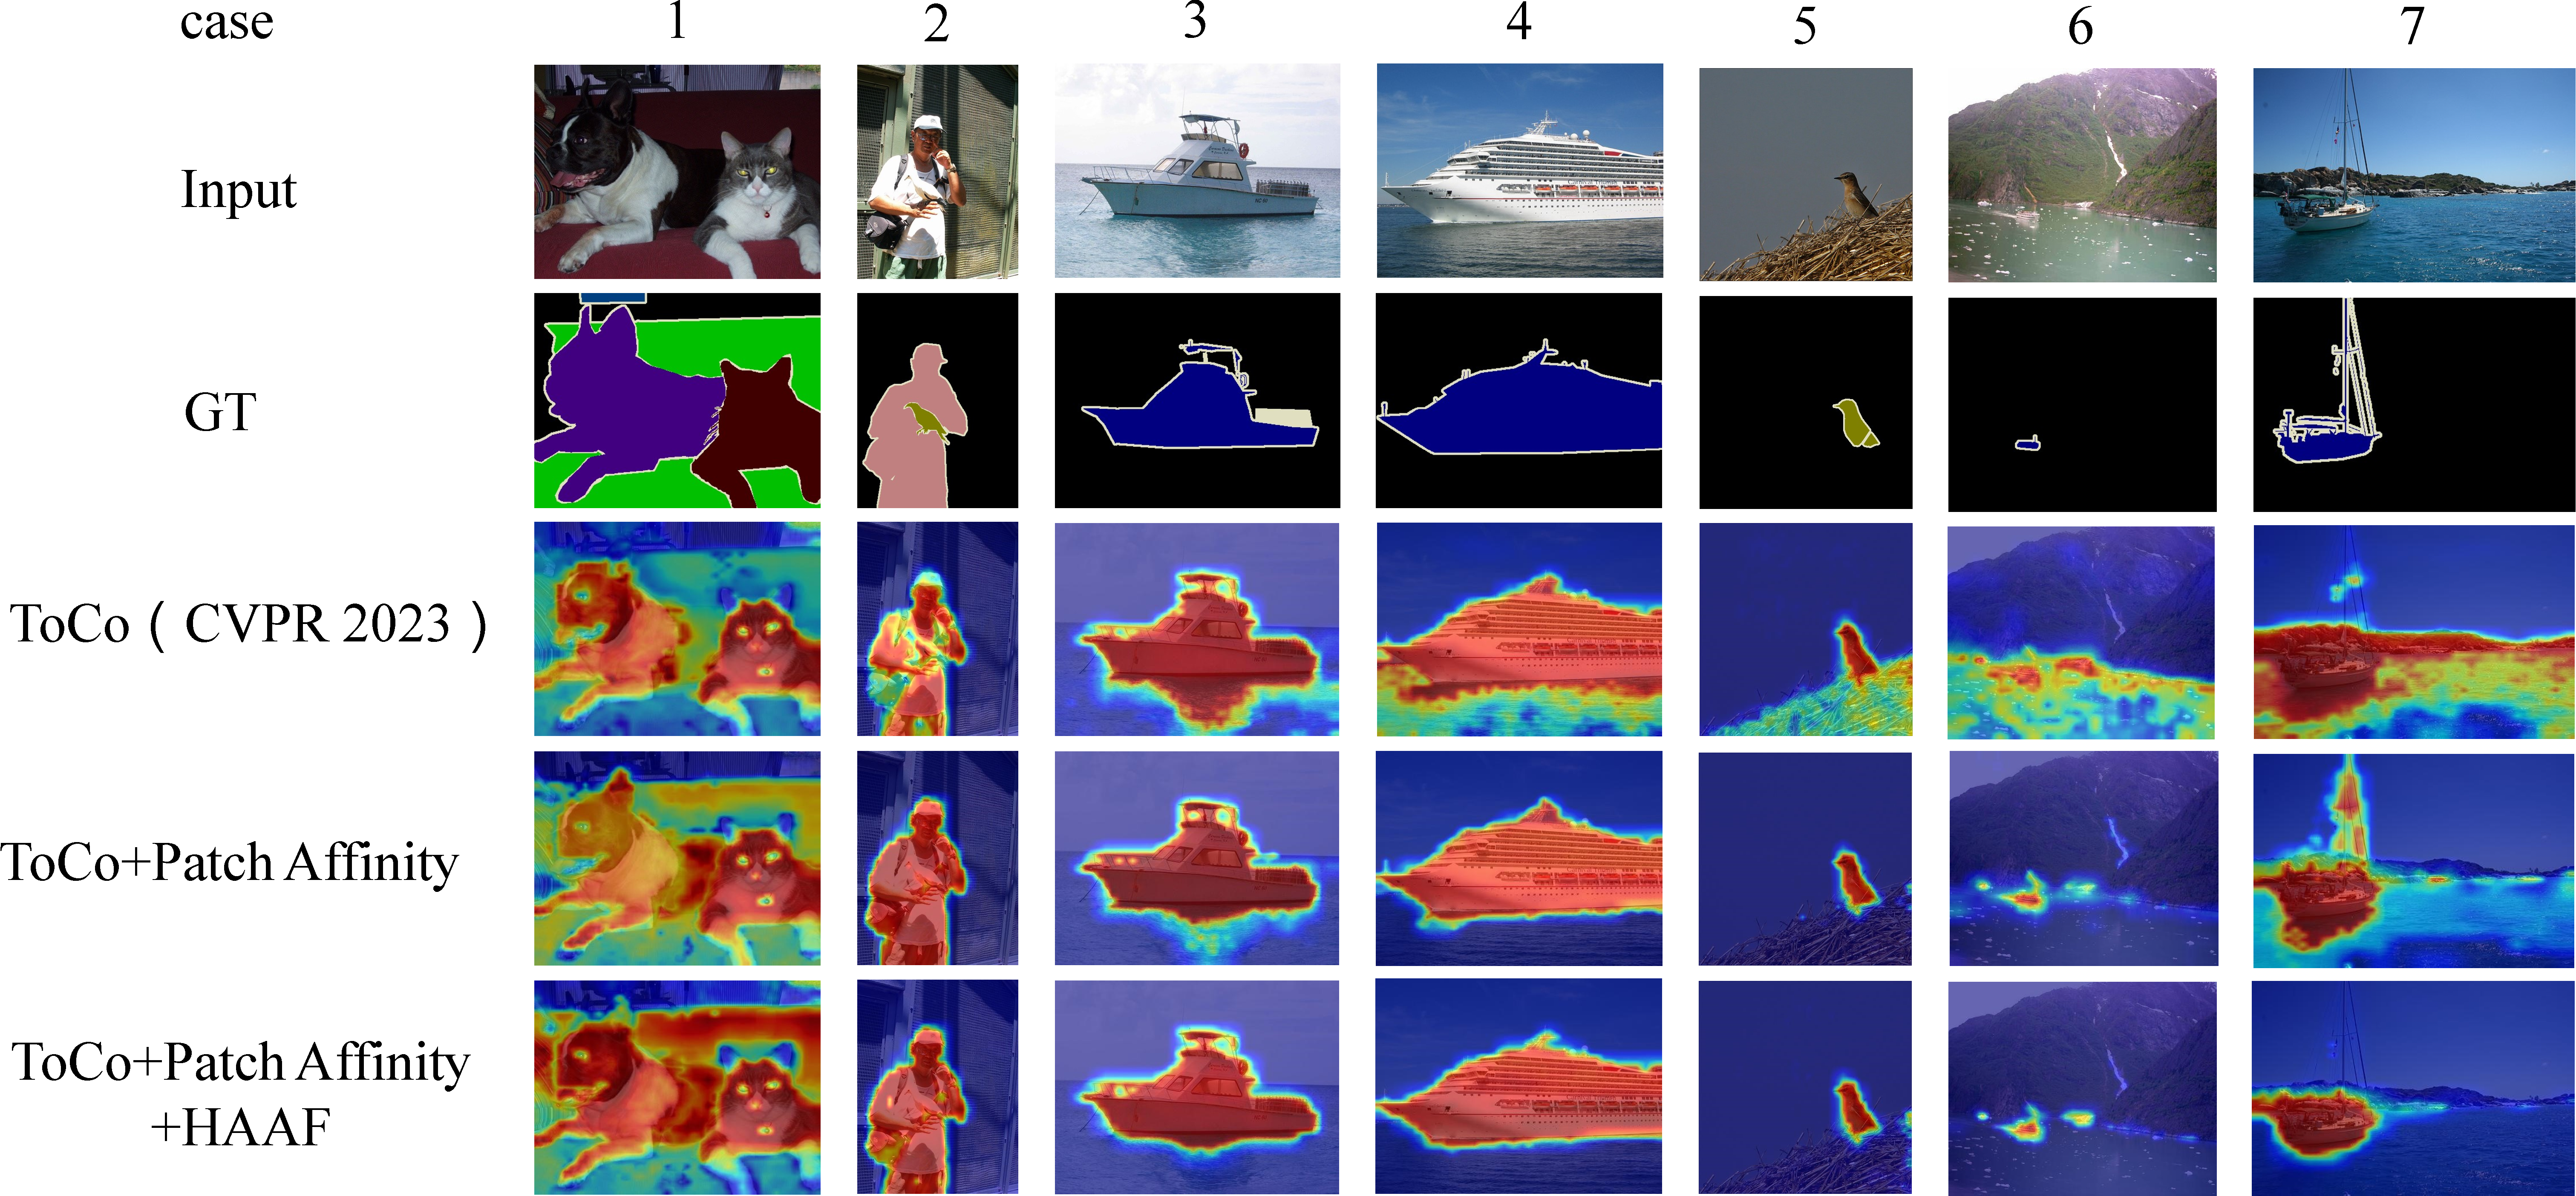
\includegraphics[width=6in]{fig/fig5.pdf}}
%     \begin{CJK*}{UTF8}{fs}
%         \caption{生成CAM可视化结果,从上到下依次为输入图片(input),真值标签(GT),ToCo生成CAM,SS-EPA生成CAM(不使用HAAF),SS-EPA生成CAM(使用HAAF)。红框部分为显著提升区域。}\label{fig5}
%     \end{CJK*}
% \end{figure*}

表\ref{table1}呈现了利用 CAM 生成伪标签的定量评估结果,在 VOC 训练集和验证集上进行评估,并与一些先进的 WSSS 方法进行比较。结果表明,本文提出的 SS-EPA 比现有的单阶段 WSSS 方法更好,且达到了与一些多阶段 WSSS 方法相当的性能。与基线方法 ToCo 相比较,无论是否使用 MS(Multi Scale) 和 CRF(DenseCRF) , SS-EPA 的性能都要优于 ToCo 。

% \begin{table}[t]
%     \setlength{\tabcolsep}{4mm}
%     \tiny
%     \centering
%     \caption{伪标签生成定量评估(MS:Multi Scale,CRF:dense CRF)(单位mIoU\%)}\label{table1}
%     \begin{tabular}{lccc}
%         \toprule
%         Method & Backbone & train & val \\
%         \midrule
%         \textbf{\textit{Multi-Stage WSSS Methods}}& & &\\
%         ViT-PCM\cite{23rossetti2022max}	& ViT-B & 67.7 & 66.0\\
%         MCTformer\cite{12xu2022multi} & Deit-S & 69.1 & -\\
%         LPCAM\cite{24chen2023extracting} & Deit-S & - & 70.8\\
%         SFC\cite{26zhao2024sfc} & ResNet101 & 73.7 & -\\
%         POLE\cite{25murugesan2024prompting} & ResNet50 & 74.2 & -\\
%         \cmidrule[0.4pt](lr){1-4}
%         \textbf{\textit{Single-Stage WSSS Methods}}& & &\\
%         RRM\cite{17zhang2020reliability} & ResNet38 & - & 65.4\\
%         1Stage\cite{27araslanov2020single} & ResNet38 & 66.9 & 65.3\\
%         SLRNet\cite{28pan2022learning} & ResNet38 & 67.1 & 66.2\\
%         AFA\cite{13ru2022learning} & MiT-B1 & 68.7 & 66.5\\
%         MCC\cite{29wu2024masked} & Deit-B & 75.1 & 72.2\\
%         ToCo\cite{03ru2023token} & ViT-B & 74.5 & 72.2\\
%         ToCo+MS+CRF\cite{03ru2023token} & ViT-B & 77.3 & 74.6\\
%         \textbf{SSEPA} & \textbf{ViT-B} & \textbf{77.1} & \textbf{74.2}\\
%         \bottomrule
%     \end{tabular}
% \end{table}
\begin{figure*}[htbp]
    \centerline{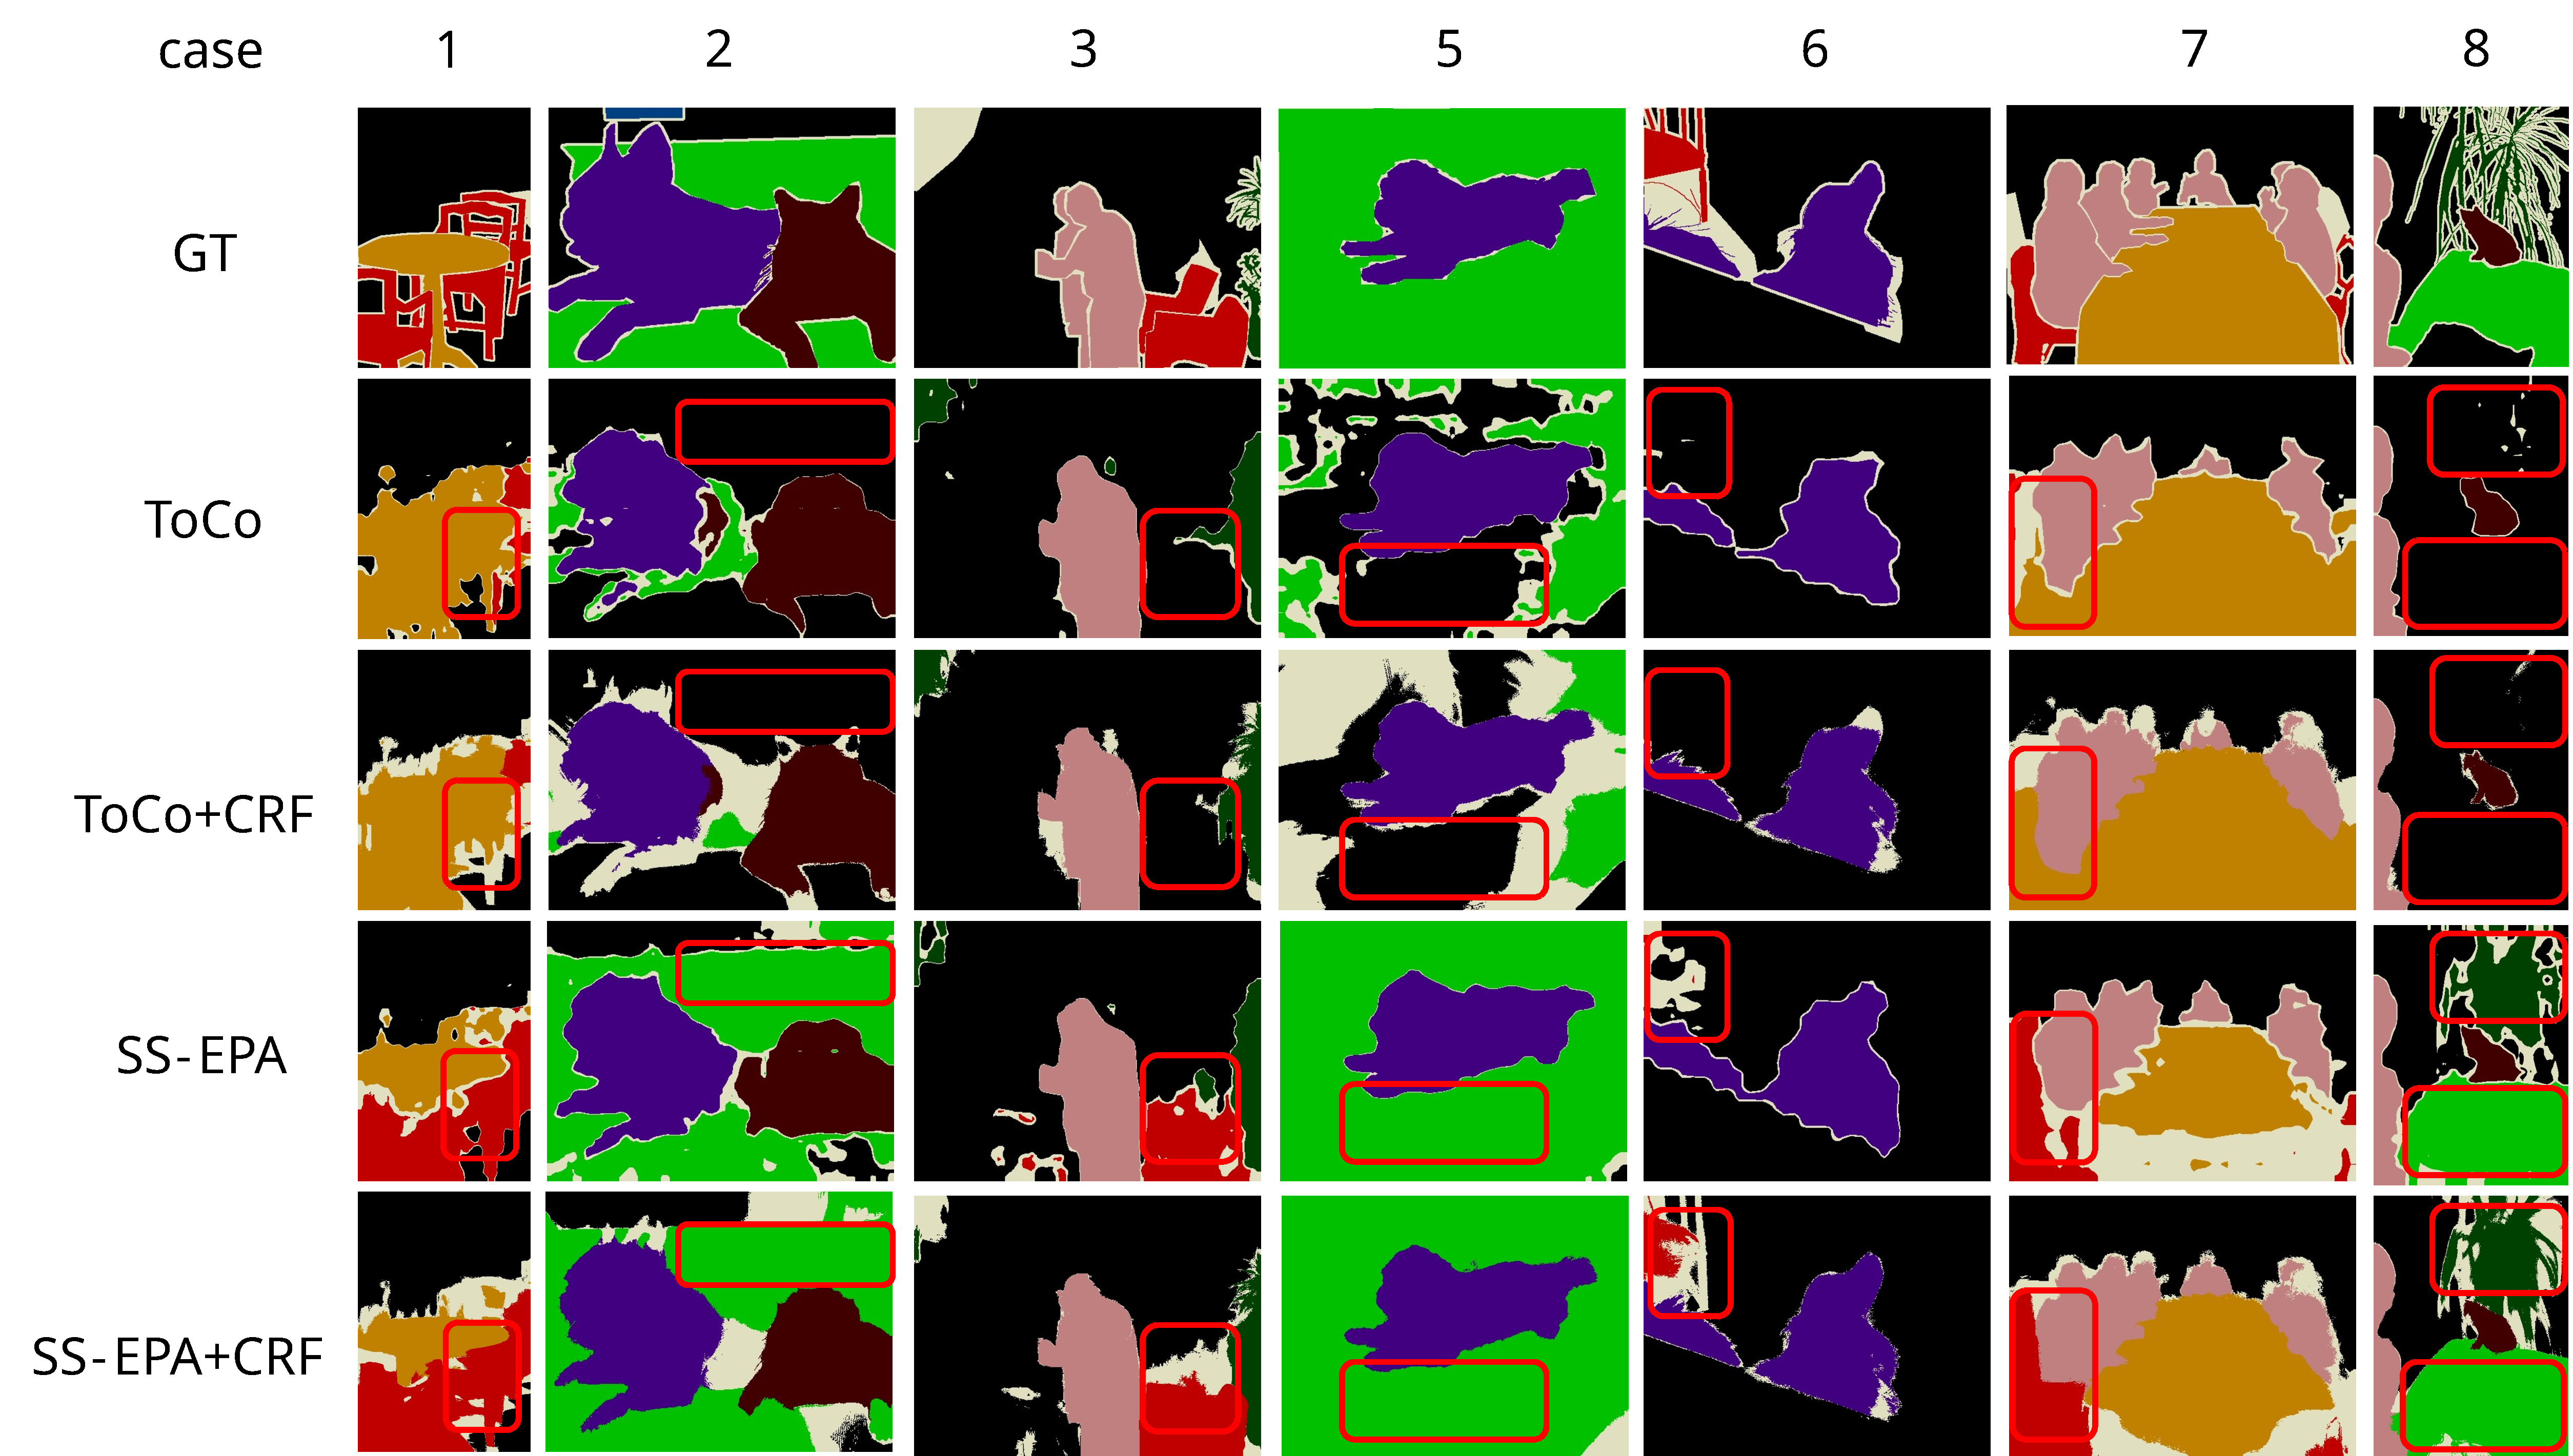
\includegraphics[width=6in]{fig/fig6.pdf}}
    \begin{CJK*}{UTF8}{fs}
        \caption{生成伪标签的可视化结果,从上到下依次为分割真值标签(GT),ToCo分割结果(不加CRF),ToCo分割结果(加CRF),SS-EPA分割结果(不加CRF),SS-EPA分割结果(加CRF)。红框部分为显著提升区域。}\label{fig6}
    \end{CJK*}
\end{figure*}

\begin{table}[htbp]
    
    \normalsize
    \setlength{\tabcolsep}{4mm}
    \centering
    \caption{分割结果定量评估(单位mIoU\%)}\label{table2}
    \tiny
    \begin{tabular}{lccc}
        \toprule
        Method & Backbone & train & val \\
        \midrule
        \textbf{\textit{Multi-Stage WSSS Methods}}& & &\\
        ReCAM\cite{33chen2022class} & ResNet101 & 68.5 & 68.4\\
        ViT-PCM\cite{23rossetti2022max }& ResNet101 & 70.3 & 70.9\\
        CLIMS\cite{08xie2022clims} & ResNet101 & 70.4 & 70.0\\
        AMN\cite{34lee2022threshold} & ResNet101 & 70.7 & 70.6\\
        EDAM\cite{30wu2021embedded} & ResNet101 & 70.9 & 70.6 \\
        SFC\cite{26zhao2024sfc} & ResNet101 & 71.2 & 72.5 \\
        POLE\cite{25murugesan2024prompting} & ResNet50 & 71.5 & 71.4 \\
        MCTformer\cite{12xu2022multi} & Deit-S & 71.9 & 71.6 \\
        L2G\cite{31jiang2022l2g} & ResNet101 & 72.1 & 71.7 \\
        BECO\cite{35rong2023boundary} & ResNet101 & 72.1 & 71.8 \\
        RCA\cite{32zhou2022regional} & ResNet38 & 72.2 & 72.8 \\
        LPCAM\cite{24chen2023extracting} & Deit-S & 72.6 & 72.4 \\
        OCR\cite{36cheng2023out} & ResNet38 & 72.7 & 72.0 \\
        \cmidrule[0.4pt](lr){1-4}
        \textbf{\textit{Single-Stage WSSS Methods}}& & &\\
        RRM\cite{27araslanov2020single} & ResNet38 & 62.6 & 62.9 \\
        1Stage\cite{27araslanov2020single} & ResNet38 & 62.7 & 64.3 \\
        AFA\cite{13ru2022learning} & MiT-B1 & 66.0 & 66.3 \\
        SLRNet\cite{28pan2022learning} & ResNet38 & 67.2 & 67.6 \\
        MCC\cite{29wu2024masked} & Deit-B & 70.3 & 71.2 \\
        ToCo\cite{03ru2023token} & ViT-B & 71.1 & 72.2 \\
        \textbf{SSEPA} & \textbf{ViT-B} & \textbf{72.4} & \textbf{73.2}\\
        \bottomrule
    \end{tabular}
\end{table}

图\ref{fig6}是 SS-EPA 生成伪标签的可视化结果,包括使用 DenseCRF\cite{22chen2014semantic} 后处理前后的结果。可视化结果表明,无论是否使用 CRF,SS-EPA 生成的伪标签在准确度上都高于 ToCo(如图6中 case 1 与case 7),且能识别到一些 ToCo 无法识别到的目标(如图6中 case 2 至 case 6 )。



\begin{CJK*}{UTF8}{zhhei}
    \subsubsection{分割结果}
\end{CJK*}

表\ref{table2}中呈现了在 Pascal VOC 2012 数据集上的定量语义分割结果,比较了本文提出的 SS-EPA 与其它的 WSSS 方法在 mIoU 分数上的表现。 SS-EPA 用ImageNet 预训练的 ViT-B(vit\_base\_patch16\_224) 作为b ackbone,在验证集和测集上分别达到了 72.4\% 和 73.3\% 的mIoU分数,比基线方法 ToCo 提升了 1.3\% 和 1.1\% 的 mIoU 分数。结果表明, SS-EPA 的性能优于现有的利用图像级标签的单阶段 WSSS 方法。此外,SS-EPA 与许多多阶段 WSSS 方法的性能相当,证明了本文所提方法的有效性。


% \begin{table}[htbp]
    
%     \normalsize
%     \setlength{\tabcolsep}{4mm}
%     \centering
%     \caption{分割结果定量评估(单位mIoU\%)}\label{table2}
%     \tiny
%     \begin{tabular}{lccc}
%         \toprule
%         Method & Backbone & train & val \\
%         \midrule
%         \textbf{\textit{Multi-Stage WSSS Methods}}& & &\\
%         ReCAM\cite{33chen2022class} & ResNet101 & 68.5 & 68.4\\
%         ViT-PCM\cite{23rossetti2022max }& ResNet101 & 70.3 & 70.9\\
%         CLIMS\cite{08xie2022clims} & ResNet101 & 70.4 & 70.0\\
%         AMN\cite{34lee2022threshold} & ResNet101 & 70.7 & 70.6\\
%         EDAM\cite{30wu2021embedded} & ResNet101 & 70.9 & 70.6 \\
%         SFC\cite{26zhao2024sfc} & ResNet101 & 71.2 & 72.5 \\
%         POLE\cite{25murugesan2024prompting} & ResNet50 & 71.5 & 71.4 \\
%         MCTformer\cite{12xu2022multi} & Deit-S & 71.9 & 71.6 \\
%         L2G\cite{31jiang2022l2g} & ResNet101 & 72.1 & 71.7 \\
%         BECO\cite{35rong2023boundary} & ResNet101 & 72.1 & 71.8 \\
%         RCA\cite{32zhou2022regional} & ResNet38 & 72.2 & 72.8 \\
%         LPCAM\cite{24chen2023extracting} & Deit-S & 72.6 & 72.4 \\
%         OCR\cite{36cheng2023out} & ResNet38 & 72.7 & 72.0 \\
%         \cmidrule[0.4pt](lr){1-4}
%         \textbf{\textit{Single-Stage WSSS Methods}}& & &\\
%         RRM\cite{27araslanov2020single} & ResNet38 & 62.6 & 62.9 \\
%         1Stage\cite{27araslanov2020single} & ResNet38 & 62.7 & 64.3 \\
%         AFA\cite{13ru2022learning} & MiT-B1 & 66.0 & 66.3 \\
%         SLRNet\cite{28pan2022learning} & ResNet38 & 67.2 & 67.6 \\
%         MCC\cite{29wu2024masked} & Deit-B & 70.3 & 71.2 \\
%         ToCo\cite{03ru2023token} & ViT-B & 71.1 & 72.2 \\
%         \textbf{SSEPA} & \textbf{ViT-B} & \textbf{72.4} & \textbf{73.2}\\
%         \bottomrule
%     \end{tabular}
% \end{table}


图\ref{fig7}展示了SS-EPA、ToCo和真实标签的分割结果。可视化结果表明,本文提出的SS-EPA成功分割了图像中的多个对象,并且与ToCo相比,SS-EPA分类的准确度更高(如图7中Val的case 1、3、4,Test的case 5、7、8),能正确发现一些ToCo中误分类为背景的前景目标(如图7中Val的case 2,Test的case 6),且整体对象边界都更加完整和准确。

\begin{figure*}[htbp]
    \centerline{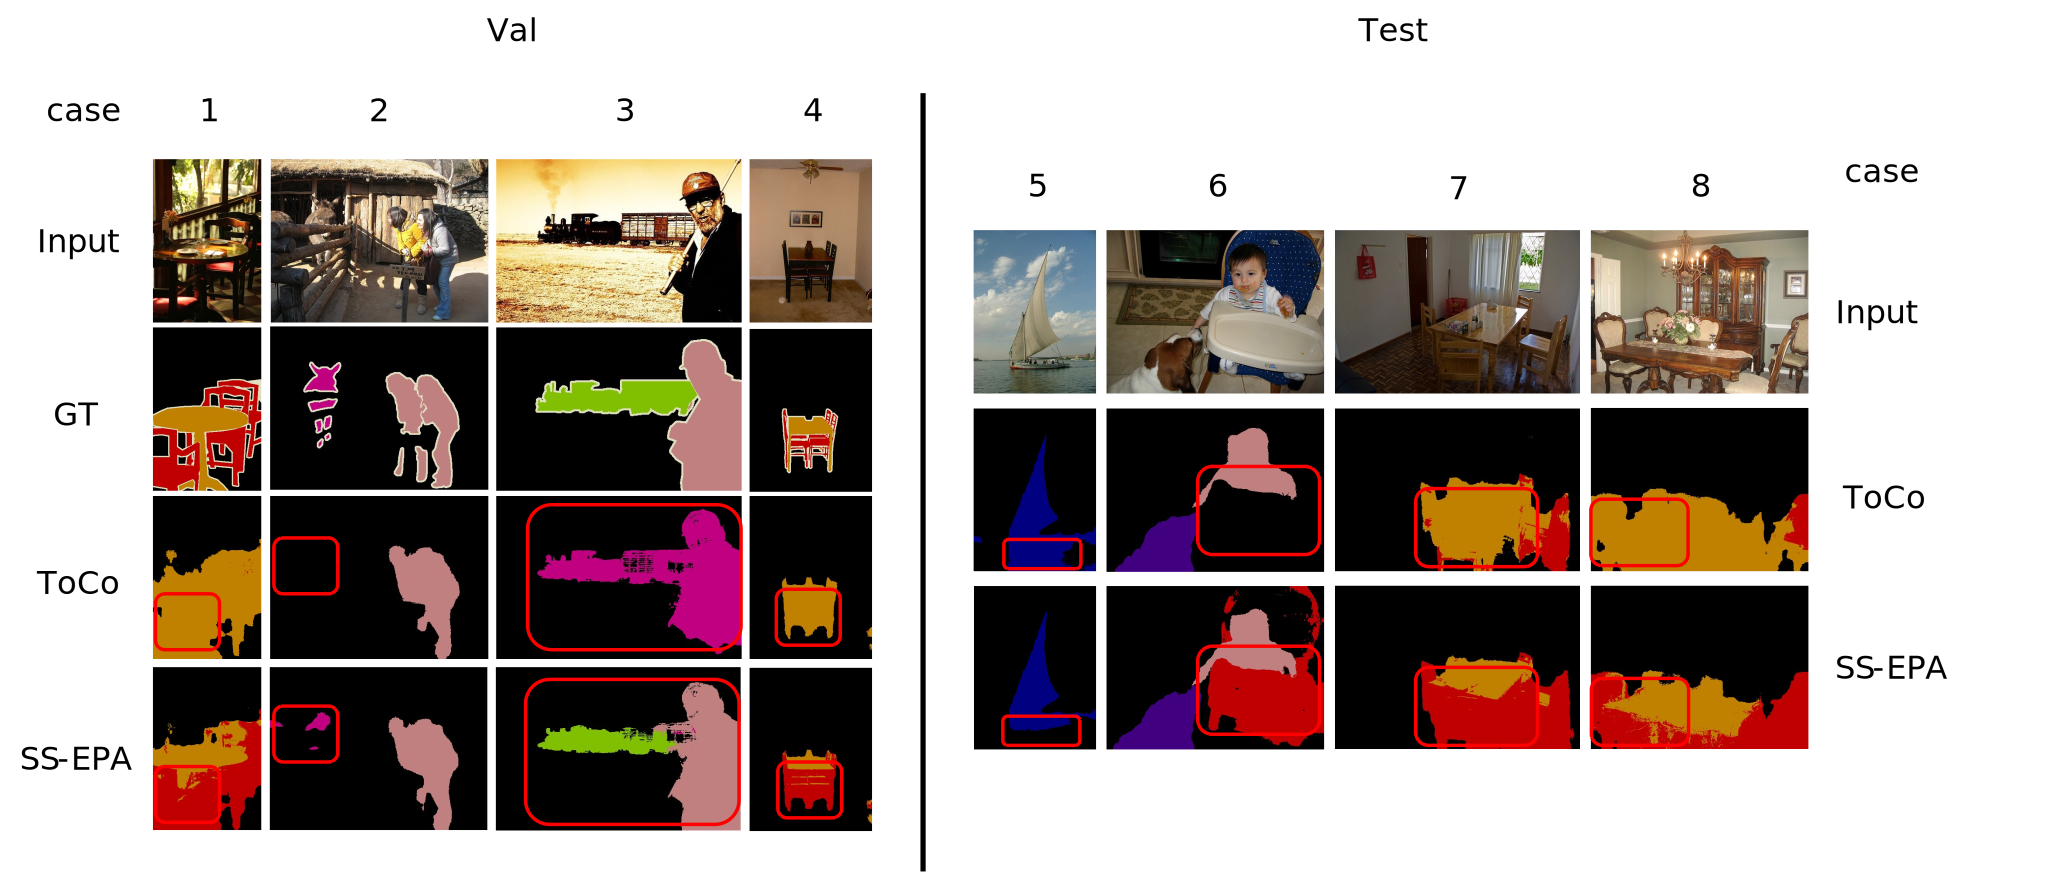
\includegraphics[width=6in]{fig/fig7_h.pdf}}
    \begin{CJK*}{UTF8}{fs}
        \caption{分割结果的可视化结果,左半部分为VOC验证集(Val),从上到下依次为输入图片(input),分割真值标签(GT),ToCo分割结果,SS-EPA分割结果。右半部分为VOC测试集(Test),从上到下依次为输入图片(input),ToCo分割结果,SS-EPA分割结果。红框部分为显著提升区域。}\label{fig7}
    \end{CJK*}
\end{figure*}


\vspace{2mm}

\begin{CJK*}{UTF8}{zhhei}
    \subsection{消融实验}
\end{CJK*}

% \begin{table*}[!htbp]
%     \small
%     \setlength{\tabcolsep}{6mm}
%     \centering
%     \caption{分割结果定量评估(单位mIoU\%)}\label{table3}
%     \begin{tabular}{lccc}
%         \toprule
%         Method & Pseudo label(train) & Seg(val) & Seg(test) \\
%         \midrule
%         ToCo & 77.3 & 71.1 & 72.21 \\
%         SS-EPA(w/o Patch Affinity) & 76.2 & 71.3 & 71.62 \\
%         SS-EPA(with Patch Affinity) & 79.0 & 71.9 & 72.73 \\
%         \textbf{SS-EPA(with Patch Affinity HAAF)} & \textbf{79.5} & \textbf{72.4} & \textbf{73.34} \\  
%         \bottomrule
%     \end{tabular}
% \end{table*}


\begin{CJK*}{UTF8}{zhhei}
    \subsubsection{补丁语义亲和力分析}
\end{CJK*}

表\ref{table3}呈现了关于伪标签和分割结果的消融实验定量评估。结果表明,使用不加HAAF增强的补丁语义亲和力后,SS-EPA可以生成更加优质的伪标签并提高分割性能。其中伪标签提升了2.8\%,分割性能在验证集和测试集上分别提升了0.6\%和1.1\%,分割的准确率更高。从图5可看出尽管在未使用HAAF的情况下存在噪声与错误,补丁语义亲和力仍有效优化了初始 CAM。

\begin{table}[!htbp]
    % \setlength{\tabcolsep}{6mm}
    \centering
    \caption{分割结果定量评估(单位mIoU\%)}\label{table3}
    \tiny
    \begin{tabular}{lccc}
        \toprule
        Method & Pseudo label(train) & Seg(val) & Seg(test) \\
        \midrule
        ToCo & 77.3 & 71.1 & 72.21 \\
        SS-EPA(w/o Patch Affinity) & 76.2 & 71.3 & 71.62 \\
        SS-EPA(with Patch Affinity) & 79.0 & 71.9 & 72.73 \\
        \textbf{SS-EPA(with Patch Affinity HAAF)} & \textbf{79.5} & \textbf{72.4} & \textbf{73.34} \\  
        \bottomrule
    \end{tabular}
\end{table}

\begin{CJK*}{UTF8}{zhhei}
    \subsubsection{HAAF分析}
\end{CJK*}

如\ref{section3.3_HAAF}节中所说,补丁语义亲和力存在噪声与错误,直接使用补丁语义亲和力并不合适。本文提出的HAAF模块显著减少了语义亲和力中的噪声和错误,并减少计算资源占用。从表3中可以看出,HAAF进一步提升了伪标签和分割结果的mIoU分数,其中伪标签提升了0.5\%,分割性能在验证集和测试集上分别提升了0.5\%和0.6\%。

\begin{table}[!htbp]
    % \setlength{\tabcolsep}{7mm}
    \centering
    \caption{SS-EPA计算资源占用实验结果评估(单位GB)}\label{table4}
    \tiny
    \begin{tabular}{lccc}
        \toprule
        Method & Backbone & Batchsize 1 & Batchsize 2 \\
        \midrule
        SS-EPA(w/o Patch Affinity) & ViT-B & 6.6 & 10.4 \\
        SS-EPA(with Patch Affinity) & ViT-B & 13.2 & 23.6 \\
        \textbf{SS-EPA(with Patch Affinity HAAF)} & \textbf{ViT-B} & \textbf{8.3} & \textbf{12.6} \\  
        \bottomrule
    \end{tabular}
\end{table}

表\ref{table4}展示了 SS-EPA 的计算资源占用评估,分别评估了 batchsize~1 和 batchsize~2 的实验结果。结果表明,在不使用 HAAF 的情况下,整个 SS-EPA 需要占据较高的的计算资源, batchsize 为 $1$ 时需要13.2GB显存, batchsize 为 $2$ 时则需要23.6GB。而 HAAF 可以将计算资源占用降低到 8.3GB 和 12.6GB ,显著减少了对计算资源的需求,提升了计算效率。

\begin{CJK*}{UTF8}{zhhei}
    \subsubsection{Backbone分析}
\end{CJK*}


表\ref{table5}展示了不同backbone下的SS-EPA和基线方法ToCo的实验结果评估。结果表明,SS-EPA在使用不同backbone的情况下比ToCo更好,在VOC验证集和测试集上的分割性能都更加优秀。其中表现最好的backbone是 vit-base-patch16-224 。与使用更高分辨率的 vit-base-patch16-384 相比,低分辨率的 vit-base-patch16-224 具有更好的泛化能力,不太容易过拟合到训练数据中的特定细节。而 vit-small-patch16-224 只有$8$层 Transformer 块,参数量和计算量都相对较少,导致其在捕捉图像中的复杂特征和细节时能力有限。

\begin{table*}[!htbp]
    \small
    \setlength{\tabcolsep}{6mm}
    \centering
    \caption{ SS-EPA不同Backbone实验结果评估(单位mIoU\%)}\label{table5}
    \begin{tabular}{lccccc}
        \toprule
        Method & Backbone & Depth & Img\_size & Seg(val) & Seg(test) \\
        \midrule
        ToCo & vit-small-patch16-224 & 8 & $224\times 224$ & 55.0 & 52.7 \\
        SS-EPA & vit-small-patch16-224 & 8 & $224\times 224$ & 57.6 & 50.2 \\
        ToCo & vit-base-patch16-384 & 12 & $384\times 384$ & 71.1 & 71.8 \\
        SS-EPA & vit-base-patch16-384 & 12 & $384\times 384$ & 71.7 & 71.9 \\
        ToCo & vit-base-patch16-224 & 12 & $224\times 224$ & 71.1 & 72.2 \\
        SS-EPA & vit-base-patch16-224 & 12 & $224\times 224$ & 72.4 & 73.3 \\    
        \bottomrule
    \end{tabular}
\end{table*}%添加实验
\begin{CJK*}{UTF8}{zhhei}
    \zihao{5}
    \vskip 1mm
    \section{结论}
\end{CJK*}

本文工作主要有以下两点:第一是提出了一种名为SS-EPA的单阶段WSSS方法,集成了端到端式多头自注意力CAM优化方法;第二是提出一种头平均注意力融合增强模块(HAAF),来进一步优化语义亲和力中的噪声和错误。具体而言,本文首先提出了SS-EPA这个单阶段WSSS方法,将端到端式多头自注意力CAM优化方法,在不影响单阶段方法的完整性和一致性的前提下,集成到单阶段WSSS框架中。鉴于语义亲和力信息包含噪声与错误,以及注意力图较为庞大,本文提出了头平均注意力融合增强模块(Head Average Attention Fusion,HAAF)。通过对注意力的不同头的权重做平均,HAAF可去除冗余信息并提高模型鲁棒性。利用多层感知机的交互能力,HAAF可以充分考虑来自不同层注意力的重要性,对包含语义亲和力的自注意力完成简化和增强。实验结果表明,SS-EPA可以显著优于其它单阶段WSSS方法,并达到与一些多阶段WSSS方法相当的性能。SS-EPA端到端式的设计,减少了中间步骤的计算和存储要求,对计算资源受限的环境更友好。
本文方法虽然取得了更优秀的分割性能,但在计算开销和局部特征学习上仍有提升空间。后续研究将骨干网络ViT更换成更加强大的 Transformer 变体如 EfficientFormer \cite{37li2022efficientformer}或 Swin Transformer \cite{38liu2021swin},通过引入高效注意力机制来进一步减少参数量和计算量,或通过滑动窗口的局部注意力来更好地捕捉局部信息。
%添加结论
% \vspace {3mm}
\zihao{5}{
\noindent \begin{CJK*}{UTF8}{zhhei}致\quad 谢\end{CJK*}\quad \begin{CJK*}{UTF8}{kai} *致谢内容.* 致谢\end{CJK*}}%添加致谢
\section{排版参考文献及引用}\label{sec:ref}

\subsection{使用bibliography排版参考文献}

编写参考文献一章是个很无聊的工作,且工作量不小。学校目前(2022年)使用的仍2005年的国标,即“GB/T 7714—2005 BibTeX Style”

模板用户需要编辑bibliography.bib文件,填写参考文献的各项属性,如title、author、year等,具体请参考\url{https://github.com/CTeX-org/gbt7714-bibtex-style#%E6%96%87%E7%8C%AE%E7%B1%BB%E5%9E%8B}。OVERLEAF网站对bibtex有比较详细的解释,如果您想要了解关于bibliography文件的基本知识,请参考\url{https://www.overleaf.com/learn/latex/Bibliography_management_with_bibtex#The_bibliography_file},其它关于bibtex的问题也可以参考该网站。其实bib文件的生成工作也可以交给zotero等文献管理软件,进一步实现参考文献管理自动化。

顺便推荐工具 Rebiber \url{https://github.com/yuchenlin/rebiber},SimBiber \url{https://github.com/MLNLP-World/SimBiber}

bib文件示例:
{
\color{green!50!black}
\begin{lstlisting}[breaklines=true,]
  @online{x1,
    title = {The Not So Short Introduction to LaTeX2e},
    year = {2021},
    author = {Tobias, O and Hubert, P and Irene, H and Elisabeth, S},
    url = {http://tug.ctan.org/info/lshort/english/lshort.pdf},
    urldate = {2021-06-05},
    langid = {english},
  }
  
  @book{x2,
    title = {LaTeX2e 及常用宏包使用指南},
    author = {李平},
    date = {2004},
    publisher = {{清华大学出版社}},
    location = {{北京}},
    langid = {中文;}
  }
\end{lstlisting}
}

示例中的x1、x2为参考文献的标识符,可以随意设定,在正文中使用\verb|\cite{x1}|命令即可实现文献交叉引用。

bib 文件编辑完成后,用户需要依次进行下面四个操作:编译 latex、编译 bibtex、编译 latex、编译 latex。2022 版编者在 Visual Studio Code 中推荐设置 Recipe

{
\color{green!50!black}
\begin{lstlisting}[breaklines=true,]
{
  "name": "XeLaTeX",
  "tools": [
    "xelatex"
  ]
},
{
  "name": "xelatex -> bibtex -> xelatex*2",
  "tools": [
    "xelatex",
    "bibtex",
    "xelatex",
    "xelatex"
  ]
},
\end{lstlisting}
}

第一项用于在没有引文变化的情况下默认编译一次 latex(耗时较短),第二项用于引文有变化的情况下使用(会比较耗时)。

如果想了解原理,请参见\url{https://liam.page/2016/01/23/using-bibtex-to-generate-reference/}。

若参考文献发生变更,或是编译发生错误,用户需要先清除.aux, .bbl, .blg文件后,重新执行以上操作。

学校规定的参考文献排版规范有一点与国标\cite{陈浩元2015GB}不同:我校要求英文人名仅首字母大写。因此模板更新了bib样式gbt7714-2005-numerical.bst,已实现仅首字母大写、其余字母小写。并且修改了文章标题单词的大小写问题,现在不会将单词首字母改为小写。

\subsection{(已弃用)thebibliography环境排版参考文献}

注释掉nuist.cls文件的第50行至第52行,并取消注释第55行至第57行,来启用thebibliography。

使用thebibliography环境来排版参考文献,代码如下:

{
\color{green!50!black}
\begin{lstlisting}[breaklines=true,]
\begin{thebibliography}{99}\setlength{\itemsep}{-0.1mm}
  \begin{spacing}{1.2}
    \zihao{-5}
    \bibitem{x1}The Not So Short Introduction to 
    \LaTeX2e \ by Tobias Oetiker, Hubert Partl, Irene Hyna and Elisabeth Schlegl.
    \bibitem{x0}李平.\LaTeX2e 及常用宏包使用指南[M].清华大学出版社,2004.
    \bibitem{x3}罗振东,葛向阳.排版软件\LaTeX 简明手册[M].第二版.北京:电子工业出版社,2003.
  \end{spacing}
\end{thebibliography}
\end{lstlisting}
}

引用文献条目时使用\verb|\ucite{}|命令,例如代码\verb|\ucite{x1}|和\verb|\ucite{x2}|就可以产生\cite{x1}和\cite{x2}上标。
%添加参考文献
% \appendix

\section*{附录}
\phantomsection
\addcontentsline{toc}{section}{附录}

\subsection*{写在后面(第一版作者)}

时间过得真快,从五一动手,到码字码到这里差不多快三天了。这么短的时间,不管模板本身还是说明文档肯定还是不够完善的。但时间所迫,也必须到这了。

有人也许行会产生疑问,word不是用着挺好的吗,干嘛要学这个,干嘛要用这个写论文呢?其实要我回答呢,的确是这样的,随便用哪个排版软件用顺手了就好了,没人强迫你做什么,关键在于自己是怎么想。

去年笔者在写学年论文时,就“吃了亏”,先是用\LaTeX 写的,生成的pdf格式的文档,但是最后学院不认,说必须用word版的,无奈后来又用word重排了一遍。(所以这里插一句,如果真有哪位朋友想用这个模板,请“严重”地考虑这个“严重”的后果,弄不好到最后,只能用它排个打印版玩玩,电子版还得word 去。)

而对笔者来说,无所谓,不是天空经常会飘来五个字儿,叫“这都不是事儿”嘛,人生本就是向死之生,要是总走直线,太快到终点了怎么办?所以人生的要义就在于走“弯路”,走得越“弯”走得越长嘛。

\subsection*{第二版修订说明}

\subsubsection*{第二版!新鲜出炉!}

两年以后\footnote{第二版修订于2017年3月13日,\url{https://github.com/LirenW/NUIST_thesis_template_V2.0}},这个模板又被重新更新了一次(原作者应该并没有更新过(因为并不能联系到原作者(sigh。因为每年的格式都会进行一些修改,所以按照现在的格式改了一下模板,特别是字号和字体,并且针对一些问题进行了修改(以下如果感觉麻烦可以略过233),不过要注意的是,NUIST一向不欢迎PDF格式的论文提交,因此此模板,正如原作者说的那样,需要慎用、慎用和慎用。\par
对于无法复制PDF的问题,由于CTeX的设置问题解决方案比较复杂,本模板采用修改字体为Adobe Song Std 的方法,不过如果要完整解决此问题请参考\url{https://www.zhihu.com/question/32207411}这个回答,不过低版本的CTeX+WinEdit套装中CTeX版本过低无法使用,可以考虑升级全部宏包(此方法可能会导致WinEdit宏包冲突,慎用)也可以等新版本的套装(听说快出了)。\par
关于行距的问题,虽然word和LaTeX的行距计算方法相同(行距:一行文字的基线(Base Line)到下一行文字的基线的距离,详见\cite{x4}),但是修改出的文章行距感觉比word略宽,不知道为什么,期待后人能解决此问题!\par

\subsubsection*{修订者的话}

说完了专业问题,聊点其他的话题好了。笔者接触LaTeX也蛮久了,从数学建模就用自己修改的模板进行论文写作,到写毕业论文时还是用LaTeX,感觉长文章基本脱离Word了,不是不会用(不自夸地说,论Word排版本人也完全可以完成长文章的各种排版工作),而是感觉Word排出来的东西一点也不美。\par
Knuth感觉自己写的东西被编辑排成了渣,于是很不开心地花时间做了个排版系统;乔布斯觉得手机太丑,于是自己做了个iPhone。我也有这种感觉,且不说Word那蛋疼的贪心断行算法(最常见的例子的是加上了数学公式和英文字符后完全不对齐的右边界)、令人抓狂的图片摆放,就拿最简单的来说,一个写作软件,为什么要让用户找不到如何更新引用!我知道那复杂的域代码和目录生成,然而一个一个设置它们的格式实在令人发指,并且一个不小心,版面就跑到十万八千里以外。不过什么是美呢?想来对我来说的话就是“Simple is the best”,能让电脑自动计算的事情完全不应该由手工来做,能动脑解决的就绝不动手。\par
世界是因为懒人才变得舒适,但“懒”往往需要的是Critical Thinking和Curiosity,而对我来说,对美这一形而上的终极目标的追求促使我探索这个世界,而对这个世界无穷无尽的美好的好奇让我在探索的过程中不太无聊。\par
引用百度百科(好吧我最唾弃百度的各种玩意了)TeX的词条的一句话吧:

\begin{quote}
  TeX是一种乐趣: 使用TeX不仅仅是一种工作手段,也是一种乐趣。它有挑战,也有荣誉。很多人在熟悉了TeX之后都开始把使用TeX作为一种爱好,而不是一件枯燥无味的劳动。
\end{quote}

我使用TeX就是因为它简洁明快,让我专注于内容而不需要纠结于无聊的排版疏忽,随意调节结构而不用担心随之而来的格式更新,总而言之就是这个样子\footnote{面白い}。\par
\subsection*{2021.6版修订说明}

\subsubsection*{南信大与PDF格式论文}

首先,笔者要和前面两位唱个反调,是时候打破“南京信息工程大学不欢迎PDF格式论文”这个传言了。南信大论文系统提交文件处写明“格式建议:word,pdf”,在笔者撰写论文前也确认过可以提交PDF格式的论文,最重要的是,笔者自己提交的就是PDF格式的论文。南信大并不是不允许PDF格式的论文。当然,笔者能够全程使用\LaTeX 撰写论文离不开笔者的毕业设计指导老师的支持,因为今年(2021年)的《关于毕业论文(设计)材料归档工作的通知》里还是写了“上传论文须WORD格式,PDF格式的论文和设计实现的系统/软件作为附件打包上传至系统。”,不过指导老师允许笔者最后的归档文件无须提交Word文档。

如果您希望使用\LaTeX 撰写论文,建议您向论文指导老师确认对\LaTeX 的态度。下面引用《关于毕业论文(设计)材料归档工作的通知》的部分段落:

\begin{quote}
    一、需归档的材料

    1、任务书;2、开题报告;3、中期检查表;4、外文翻译;5、毕业论文定稿(word和PDF格式);6、指导教师审阅意见表;7、系统或其他附件

    二、归档要求

    所有材料的电子版均需保存或上传到“毕业设计(论文)智能管理系统”(下称“系统”)
    注:1、上传论文须WORD格式,PDF格式的论文和设计实现的系统/软件作为附件打包上传至系统。如果是软件,还需要写一份软件说明书,说明具体的操作步骤;如果是硬件,建议将硬件保留下来,将硬件演示过程拍一段视频,上传至系统。
\end{quote}

\subsubsection*{更新说明}

本次修订\footnote{网址:\url{https://sakronos.github.io/NUIST_Bachelor_Thesis_LaTeX_Template/}}根据南信大2021年本科毕业论文格式要求对原有模板进行修订,参考了《南京信息工程大学LaTeX毕业论文模板V3.1》\cite{geiNanJingXinXiGongChengDaXueLaTeXBiYeLunWenMoBanV31GengXinWuXuYiLaiCTeXRuanJian2021}。关于页码、声明页、按章编号等《南京信息工程大学本科生毕业论文(设计)撰写排版规范》没有提及的额外排版要求则是根据笔者导师要求设定的,如果与您所在学院老师要求发生冲突,请报告。

由于时间较长,笔者无法一一列出本次修改的具体内容,这里根据记忆尽量列出修订内容:
\begin{enumerate}[1、]
    \item 调整了几处字体大小
    \item 将图片、表格、公式设置为按章编号
    \item 添加了声明页
    \item 设置了页码
    \item 使用GB/T 7714—2015 BibTeX Style排版参考文献
    \item 限定模板使用的字体为SimSun、SimHei、SimKai和Times New Roman
    \item 替换已弃用的宏包和命令
    \item 更新\verb|\thanking|命令,添加\verb|\forthsection|命令
    \item 将\verb|\linespread|设置为1.335,以得到更接近MS Word下多倍行距1.25的效果
    \item 图片编号与图片标题间的分隔符设置为空格
    \item 更新模板介绍(本PDF文档)
\end{enumerate}

笔者在使用本模板的过程中没有遇到“文字无法复制的问题”,如果有同学遇到该问题请报告。

\subsubsection*{闲话}

虽然很讨厌写字,但是笔者还是写一点闲话吧。

不像该模板的创建者和第一位修订者,笔者之前并没有使用\LaTeX 的经验。笔者是在写论文的过程中不断摸索\LaTeX 的使用方法,对\LaTeX 的了解很少,因此笔者怀着诚惶诚恐的心情修订这份模板。各位如果能指出模板和本文中的错误,笔者会非常开心的。笔者也期待各位加入本模板的修订工作,笔者的文字功力太差,难免写出晦涩难懂的语句,需要各位帮助补充/润色模板文档。

下面是吐槽,Windows 系统下的TeX Live Manager这个图形化工具做的很是不好,更新Packages时不能最小化。刚刚笔者用Windows的显示桌面强行最小化这个工具后,无法还原到桌面了!!!笔者现在不知道更新的进度,只能等它在后台更新完……以后还是老老实实地用命令行更新了。(现在发现能用任务管理器强行最大化TeX Live Manager)

\subsubsection*{致谢}

本次修订首先要感谢本模板的制作者和2.0版修订者,如果没有这两位的工作,我不会鼓起勇气使用\LaTeX 撰写毕业论文,本次修订也是在这两位的工作基础上进行的。

然后,感谢我的毕业论文指导老师,感谢老师指出论文排版不美观的地方,帮助我改进该模板。

最后,感谢《南京信息工程大学LaTeX毕业论文模板V3.1》的制作者。虽然本次修订工作与这位的算是各自进行,但是您的工作给了我不少启发,也激励我在提交论文后继续完善本模板。您的CLS文件层级分明,值得学习。遗憾的是您留下的邮箱地址不存在,无法与您取得联系。
\subsection*{2022版修订说明}

\subsubsection*{更新内容}

\begin{enumerate}[1、]
    \item 封面信息允许换行,以免遇到如“计算机学院 软件学院 网络空间安全学院”这样实在写不下的学院名称
    \item 解决参考文献作者全部大写的问题、解决标题单词首字母被改为小写的问题
    \item 注释号采用六角括号
    \item 公式序号使用中文括号
    \item 更改行距换算
    \item 增加 algorithm 和 algorithmic 包排版伪代码
    \item 使用 \verb|\paragraph| 代替 \verb|\forthsection|
    \item 修复参考文献标题上方过多的空白
    \item 修改摘要页格式(边距、空行)
    \item 减小参考文献列表项的间距
\end{enumerate}

%添加附录
% \zihao{5}
\noindent \textbf{Background}

\zihao{5-}{
\setlength\parindent{2em}
*论文背景介绍为\textbf{英文},字体为小5号Times New Roman体*

论文后面为400单词左右的英文背景介绍。介绍的内容包括:

本文研究的问题属于哪一个领域的什么问题。该类问题目前国际上解决到什么程度。

本文将问题解决到什么程度。

课题所属的项目。

项目的意义。

本研究群体以往在这个方向上的研究成果。

本文的成果是解决大课题中的哪一部分,如果涉及863$\backslash
$973以及其项目、基金、研究计划,注意这些项目的英文名称应书写正确。}
%添加项目与背景介绍

\end{CJK*}
\end{document}


